With a deeper understanding of the historical Jesus, the interpretation of the events that followed his death can change quite dramatically as well.

In the context of an influential royal figure with a large following and with early texts in circulation, the early Christian movement can be seen in a new light.

If we acknowledge that Jesus was framed in Greek and Egyptian royal cult, then Christianity appears from the very beginning as an extension of that tradition.
Jesus did not emerge in a vacuum with completely new ideas.
He was a continuation of the recently fallen Greek empire and inherited a movement that already spanned a major part of Rome.

In this chapter we will try to view the events of the New Testament after Jesus’ death in the light of what we found in previous chapters.
As the Gospel of Matthew closes: πορευθέντες οὖν μαθητεύσατε πάντα τὰ ἔθνη --- “Go, therefore, and make disciples of all nations.”

\section{Who were the gentiles?}\label{sec:who-were-the-gentiles}

The word “gentiles” has long been misapplied in the context of the New Testament.
It is almost universally taken to mean “anyone who is not Jewish.”
The confusion comes from the Hebrew word \texthebrew{גּוֹיִם} (\textit{goyim}), which in many contexts does carry this meaning.
While in the Septuagint, \textit{ethnē} often is used as a translation of \texthebrew{גּוֹיִם} (\textit{goyim}), it does not show any sign of the same meaning in the context of the New Testament or other Hellenistic works and inscriptions.
The key point missed by most interpreters is that \textit{panta ta ethnē} does not refer to \texthebrew{גּוֹיִם} (\textit{goyim}) or to all peoples universally, but to the nations of the Greek world.
In Hellenistic inscriptions, the phrase “all the nations” (\textit{panta ta ethnē}) is repeatedly used for the \textit{oikoumene}, the civilized world subject to the emperor.
It was imperial language, not global anthropology.
Thus, Matthew’s Great Commission is not an open-ended summons to the Americas or India, but to the Greek-speaking nations of the empire.

Καὶ εὐλογηθήσονται ἐν τῷ σπέρματί σου πάντα τὰ ἔθνη τῆς γῆς --- “And in your seed all the nations of the earth shall be blessed” (Gen 22:18 LXX).
This verse is quoted in Galatians 3:8 to argue that “all the nations” were meant to be part of God’s covenant.
Here the nations are not portrayed as outsiders, but as peoples folded into God’s promise.

Βασιλεῖς τῆς γῆς καὶ πάντες λαοὶ, ἄρχοντες καὶ πάντες κριταὶ γῆς… ὕμνος πᾶσι τοῖς ὁσίοις αὐτοῦ, τοῖς υἱοῖς Ἰσραήλ, λαῷ ἐγγίζοντι αὐτῷ --- “Kings of the earth and all peoples, rulers and all judges of the earth… a hymn for all His saints, the sons of Israel, a people near to Him” (Ps 148:11, 14 LXX).
The kings and peoples of the earth are included in God’s rule, yet the focus remains on Israel as the center.

The same idiom appears in imperial decrees, for example in the already cited Priene calendar inscription (9 BC), which describes the birthday of Augustus as “gospel for all the nations,” clearly referring to the subjects of the empire rather than to the entire globe.

“All the nations” in these texts does not mean “non-Jews.”
It refers to all peoples under God’s sovereignty, which in a Hellenistic and imperial context meant the nations integrated into the covenantal and political order of the \textit{oikoumene}.
That included Jews as well as Greeks and others within the world of the recently fallen Greek empire.

\section{Are Acts a work of fiction?}\label{sec:are-acts-a-work-of-fiction}

The Acts of the Apostles describes the actions of the apostles after Jesus' ascension through Paul's Roman custody, ending around 60--62 AD.
It follows the travels of Paul and Peter to all the major cities of the former Greek empire, and describes the interactions of the apostles with the church authorities there.
The Acts of the Apostles is often dismissed as a work of fiction.
And indeed, if Acts are read as a history of the spread of a new religion, we already run into major contradictions.
Most notably the churches described in Acts and the epistles appear fully formed, with no indication of how they were established.
There is actually very little in the way of religious conversion in there.
Educated Greek discourse already spoke in ``highest god'' terms, and Acts depicts Paul exploiting this register when he addresses the Athenian elite about the ``unknown god.''
A lot of the speeches in Acts are clearly political speeches, and while there are certainly some religious elements to them, they do not resemble the speeches of a religious missionary.
It is always argued that to be an effective missionary, one must first establish a rapport with the audience, and so describe the local beliefs and then show how the new religion is compatible with them.
And so the definition of God as the omnipotent force behind the universe, who created everything, and who is not confined to a temple, is a perfect fit for the Hellenistic monotheism that was already present in the former Greek empire.
To wit, during the episodes in Ephesus, where there is a strong cult of Artemis, and physical idols, Paul does attack the beliefs directly.
So this looks like praising the modern ideas of Greek faith and denouncing the old ones, not trying to find commonalities between Judaism and the whatever the local beliefs were.

Once we understand more clearly what apostles and churches were, the Acts of the Apostles makes a lot more sense.
For centuries apostles have been emissaries of centralized state and ecclesia is the civic assembly of the city, local government.
These were not religious terms but administrative ones.
We have well-developed councils, bishops, deacons and treasuries.
This makes absolutely no sense if we assume this is a formation of a new church with a handful of members.
It makes a lot of sense if we remember all of this already existed as part of the Greek civic order, and the apostles were simply trying to maintain the existing order under a new reality of Roman rule.
In that light the Acts of the Apostles is a record of trying to maintain the Greek civic order under a new reality of Roman rule.
There are many references to acts of recommendation, letters of introduction, confiding common law between the ecclesia of different cities, and numerous references to newly appointed officials.
After the conquest and the rebellions, the texts were indeed altered to account for a failed rebellion rather that a failed prophecy of the end of the world.

Like we see clear additions in the gospels that are often dated to 70 AD or shortly after, we can suspect that the Acts of the Apostles were written at the time of the edits.
We are looking here at the second generation of Greeks and Jews under direct and harsh Roman rule coming to terms with the reality of failed rebellions.

\subsection{What is quite striking is that Paul and others write to so many different churches over the short period of time.}\label{subsec:what-is-quite-striking-is-that-paul-and-others-write-to-so-many-different-churches-over-the-short-period-of-time.}

There is a major challenge for the traditional timeline of the apostles establishing so many churches in such a short period of time.
These churches would have to all be established, grow, keep up to date with the fastly shifting theology, and then do nearly nothing for the next 100 years.
These churches immediately showed up in every single major city in the former Greek empire, and no churches showed up anywhere else.
All of the correspondence and scripture was written in Greek, and no other languages.
It is important to point out that Greek was absolutely not the lingua franca in any part of the Roman empire that was not recently part of the Greek empire.
The lingua franca of the Roman empire was Latin, and that was the only language that was used in the administration and the primary language used by the authors.
If the apostles were to establish churches everywhere in the Roman empire, and not just in the former Greek empire, then we would have had the epistles to the extremely prominent cities of Mediolanum, Lutetia, Aquilea, Lugdunum, Memphis, and Londinium.
The truth is that no matter how we model the growth of the early church, it is not possible to explain the patterns we observe.

Even more striking is the total absence of Aramaic or Hebrew letters.
If the apostles' mission were Jewish in nature, at least some correspondence would survive in the languages of Judea.
Instead, all the letters are in Greek, to Greek assemblies, proving that the movement was imperial and Hellenistic at its core.
The same institutional pattern running through Acts becomes unmistakable in Paul's own letters, which operate not as private devotions but as imperial circulars to Greek civic assemblies.

\subsection{Paul as Imperial Envoy and Administrator}\label{subsec:pauls-letters-as-state-correspondence.}

Paul's letters read like circular correspondence from a royal chancery, not like private notes to small devotional groups.
He addresses \textit{ekklesiai}, the same civic assemblies that governed Greek cities, and he orders public reading, courier circulation, and inter-city dissemination exactly as administrative circulars were handled.
His greetings from co-workers function like official co-signatories, and his directives on discipline, finance, and adjudication mirror the instructions sent from higher authority to subordinate poleis.
This is the epistolary footprint of an imperial envoy issuing policy, not of a village preacher sending pious advice.

\subsection{Paul's Letters as Executive Correspondence}\label{subsec:pauls-letters-as-executive-correspondence}

Some scholars dismiss portions of the Pauline corpus as forgeries on the basis of stylistic and theological variation.
That judgment rests on a modern literary model that equates authorship with uniform personal prose.
The letters themselves contradict this model at the level of explicit evidence.
Romans 16:22 names Tertius as the physical writer, directly separating authority from penmanship.
Paul's autograph formulas appear as ratification marks, not as claims of total composition.
``I, Paul, write this greeting with my own hand'' functions as formal approval of a completed document (1 Cor 16:21, Gal 6:11, Col 4:18, 2 Thess 3:17).
Such authentication is precisely how delegated correspondence was validated in the ancient world.
Greek and Roman elite figures did not draft letters line by line.
Strategoi, envoys, and league officials issued instructions orally and entrusted composition to staff.
Assistants shaped vocabulary, sentence structure, and rhetorical polish within an approved policy framework.
This administrative model predicts stylistic variation across authorized letters.
A single dictator would produce stronger stylistic uniformity than the Pauline corpus exhibits.
Paul's named associates function as operational staff rather than devotional companions.
They carry letters, manage funds, arbitrate disputes, and represent Paul in person.
By ancient standards, a letter drafted by authorized staff fully embodied the sender's identity and authority.
If Paul supplied direction, policy, and approval, the resulting letters were unambiguously Pauline.
The division between ``authentic'' and ``deutero-Pauline'' letters therefore rests on an anachronistic definition of authorship.
No ancient reader would have regarded an authorized Pauline letter as a forgery.

His political profile matches the letters.
He appeals to Caesar as a Roman citizen.
He travels through the network of Greek poleis that once formed the backbone of Alexander's empire.
His address in Athens (Acts 17) is a philosophical-diplomatic speech pitched at elites, not a sectarian sermon.
Acts frames him as the authorized representative of the Christ-emperor to the cities of the Greek world.

His vocabulary confirms the administrative register.
He lists \textit{thronoi}, \textit{kyriotētes}, \textit{archai}, and \textit{exousiai} as if reading a court hierarchy (Col 1:16; Eph 1:21).
\textit{Thronoi} are sovereign seats of rule.
\textit{Kyriotētes} are lordships with jurisdictional dominion.
\textit{Archai} are magistracies and command offices.
\textit{Exousiai} are delegated legal powers to act and enforce.
Christ is enthroned ``at the right hand'' above every such office (Eph 1:20--21).

His military language is constitutional, not mystical.
``Share in suffering as a good soldier of Christ Jesus'' is enlistment into imperial service (2 Tim 2:3).
``The armor of God'' equips troops of the king, not metaphorical pietists (Eph 6:10--17).
``I bear the stigmata of Jesus'' marks the branded body of a sworn man (Gal 6:17).
``Sealed with the Spirit'' identifies the bureaucratic seal of a new jurisdiction (Eph 1:13).
``Jesus is Lord'' is an oath of allegiance, not a devotional slogan (Rom 10:9).
Stoic writers use soldier-language for private discipline, but they never combine it with branding, sealing, thrones, officers, and assemblies.
Paul does.
His military terms sit inside a full administrative register, where stigmata mark jurisdiction, seals record enrollment, and ``Lord'' functions as an oath rather than a slogan.
This cluster has no parallel in philosophical moralism; it belongs to the machinery of allegiance and governance.

The civic layer is explicit.
``Our \textit{politeuma} is in heaven'' declares citizenship in a capital city with its own law (Phil 3:20).
\textit{Episkopoi} and \textit{diakonoi} are administrative offices---overseers and service officials of a civic body (Phil 1:1).
``God has appointed, first apostles, second prophets, third teachers\ldots'' is rank ordering, not mystical taxonomy (1 Cor 12:28).
``The saints will judge the world'' grants appellate competence to the citizen body (1 Cor 6:2--3).

Once you see the court chart and the civic map, Paul's silence on Jesus's daily sayings stops being a problem.
He is promulgating a constitutional charter for a restored empire, not composing a biographical memoir.

\subsection{Ekklesia --- the civic assembly continued}\label{subsec:ekklesia-the-civic-assembly-continued}

The word ἐκκλησία (\textit{ekklēsía}) did not name a new religious club.
It was the same civic assembly that governed the Greek city before the Roman conquest.
It was the same sovereign body of citizens that passed laws, heard proclamations, and received official dispatches.
After conquest the population and magistrates sought continuity, not reinvention.
They kept their assemblies, their procedures, and their language.
Only the allegiance changed.
The assembly now recognized the rightful \textit{Christos} instead of Rome.
This is why all the correspondence is in Greek.
This is why the addressees are the historic poleis of the Greek world.
Paul is not inventing a “church.”
He is addressing the standing political assemblies of the Greek cities as they realign themselves to the true king.

As established in Chapter 2, the ecclesia was not merely a religious gathering but the governing body of the Greek city, complete with civic offices, governance procedures, and social functions.
The epistles confirm this institutional continuity at every level.

\subsubsection{Diakonoi and episkopoi: civic offices already functioning}\label{subsubsec:diakonoi-and-episkopoi-civic-offices-already-functioning}

Paul's earliest letters do not introduce new offices; they address existing ones.
Philippians 1:1 (written c.~60--62 AD) opens: ``Paul and Timothy, servants of Christ Jesus, to all the saints in Christ Jesus who are at Philippi, with the \textit{episkopoi} and \textit{diakonoi}'' (overseers and deacons).
This is a standard civic salutation.
Paul does not explain what these offices are because the Philippian assembly already knows: they are the same officials who managed the civic assembly before.

Romans 16:1 (c.~57 AD) commends Phoebe as a \textit{diakonos} of the assembly at Cenchreae.
She is not a volunteer; she holds an administrative office, the same office documented in Greek civic assemblies and temple complexes for centuries.
Epigraphic evidence makes this continuity concrete rather than rhetorical.
The Erythrai decree (AIO 296, fifth century BC) names \textit{episkopoi} as civic magistrates who ``allot and install the Council,'' establishing the title within formal political administration.
A statue base on the Athenian Acropolis (IG II² 3464) honours Syeris, \textit{diakonos} of the priestess Lysimache, showing the office embedded in the state cult of Athena Polias.
Jewish diaspora---the communities of Jews living outside their traditional homeland in Palestine---inscriptions from Asia Minor list \textit{gerousiarch}, \textit{grammateus}, and \textit{diakonos} together as standard communal offices, demonstrating that \textit{diakonoi} belonged to the wider Hellenistic administrative vocabulary, not a Christian invention.
Inscriptions from Termessos and Mylasa attest an \textit{ekklesia kyria} still active under Roman rule, proving that the civic assembly remained a functioning institution in the first century.
Later material from Messene shows the same trajectory: a classical assembly hall remodeled in the fourth century by \textit{episkopos} Theodoulos, whose donor inscription lies in the mosaic floor, marking the literal takeover of civic space by Christian officers.
The Pastoral Epistles (1 Timothy 3:1--13) later codify qualifications for \textit{episkopoi} and \textit{diakonoi}, but these read as regulations for \emph{existing} offices, not as the invention of new ones.
The complexity and specificity---managing households, financial integrity, temperance---presume an established administrative role, not a blank slate.

Chapter 2 demonstrated that \textit{diakonoi} managed communal meals in Greek assemblies, assisted in temple rites, and served in Hellenistic cults (including Isis and Serapis).
Paul's letters confirm these exact functions: \textit{diakonoi} handle financial collections (2 Corinthians 8--9), coordinate logistics, and serve at communal meals (1 Corinthians 11).
These are civic stewards continuing their institutional role under a new sovereign.

\subsubsection{Civic governance procedures in the epistles}\label{subsubsec:civic-governance-procedures-in-the-epistles}

The epistles employ the full vocabulary of Greek civic administration.
Philippians 3:20 declares ``our \textit{politeuma} is in heaven.''
\textit{Politeuma} is not ``citizenship'' in the abstract; it is civic enrollment, the register of a political community with jurisdiction and legal standing.
Paul is asserting that the Philippian assembly's true civic authority derives from the heavenly king, not from Rome.

Romans 13:1 and Colossians 1:16 use \textit{archai} and \textit{exousiai}---magistracies and jurisdictions---the same terms employed in civic decrees and imperial administration.
These are not mystical concepts; they are constitutional offices.
Paul treats them as such, mapping the believers into a bureaucratic order under Christ as supreme magistrate.

Financial administration appears immediately and in detail.
1 Corinthians 16:1--4 instructs the assembly to organize a collection, appoint delegates, and transfer funds to Jerusalem.
2 Corinthians 8--9 describes inter-city financial coordination, accountability measures, and competitive giving between assemblies.
This is civic governance, not personal charity.
It presumes treasuries, ledgers, and auditing procedures---the infrastructure of the Greek assembly.

Public reading protocols mirror civic procedure.
1 Thessalonians 5:27: ``I charge you by the Lord to have this letter read to all the brothers.''
Colossians 4:16: ``When this letter has been read among you, have it also read in the assembly of the Laodiceans, and see that you also read the letter from Laodicea.''
These are the circulation and public reading protocols of official civic circulars, not private correspondence.
Paul is issuing decrees to be proclaimed in assembly and exchanged between cities, exactly as a Greek magistrate or royal emissary would.

\subsubsection{Sociological continuity: status, factions, and the civic catwalk}\label{subsubsec:sociological-continuity-status-factions-and-the-civic-catwalk}

Chapter 2 demonstrated that the Greek ecclesia served a sociological function: it was the primary venue for status display, where families dressed their best, displayed wealth, and enacted social hierarchy.
Ancient sources---Aristophanes, Demosthenes, Athenian scholia---mockingly describe ``overdressed youths'' and citizens ``showing off garments and jewelry'' at civic gatherings.
The epistles confirm this behavior continued without interruption.

1 Corinthians 11:17--34 describes the communal meal at Corinth: the rich arrive early, consume the food and wine, and leave the poor with nothing.
Some are hungry; others are drunk.
Paul condemns this not as a new problem but as a violation of the assembly's purpose.
The theological dispute is riding on sociological rails inherited from the civic assembly.
The assembly has become a venue for economic competition and status performance, exactly as it functioned in the Greek civic context.

1 Corinthians 11:2--16 addresses head coverings and appearance during assembly.
This is not about piety; it is about public presentation.
The debate over veiling, hairstyles, and gendered appearance makes sense only in a context where the assembly functions as a civic stage, where participants are seen and judged.

James 2:1--7 condemns favoritism toward the rich: ``Suppose a man comes into your assembly wearing a gold ring and fine clothes, and a poor man in shabby clothes also comes in.
If you show special attention to the man wearing fine clothes... have you not discriminated?``
This scenario presumes the assembly is a place where economic status is displayed through clothing and jewelry, where social comparison is constant, and where deference to wealth is a live temptation.
This is the Greek civic assembly in operation.
Notably, gold rings and reserved seating by status are Greek civic markers, not distinctively Jewish; first-century diaspora synagogues themselves adopted Greek governance structures (archons, gerousia, grammateis), functioning as polis-style civic groups within the Hellenistic world.

1 Corinthians 1:10--17 describes factions: ``I follow Paul,'' ``I follow Apollos,'' ``I follow Cephas.''
This is not only sectarian theology but also civic faction politics.
Greek assemblies were notorious for splits along patronage lines, with rival orators attracting competing blocs.
Paul's Corinthian assembly exhibits the same dynamic, because it \emph{is} the same institution, operating under the same social logic.

The assemblies did not need to \emph{learn} how to have factions, manage money, read decrees aloud, display status, or appoint officials.
They already knew, because they had been doing it for centuries.

\subsubsection{Institutional complexity appears instantly: not evolution but continuation}\label{subsubsec:institutional-complexity-appears-instantly-not-evolution-but-continuation}

Traditional models assume early Christianity began as a handful of believers in house meetings and gradually developed institutional structures over generations.
The epistles refute this.
Moreover, references to house meetings appear in \emph{later} epistles (Romans 16:5, Philemon 1:2, Colossians 4:15), suggesting that the shift to household gatherings reflects increasing Roman surveillance rather than the original institutional form.
As Roman rule strengthened and political assemblies came under closer scrutiny, some meetings moved to more covert locations.
This is evidence \emph{for} political continuity---assemblies forced underground by imperial crackdown---not evidence against it.
The behavior described remains empirically civic: factions, financial systems, status display, and inter-city coordination.
1 Corinthians, written c.~54--55 AD---only twenty to twenty-five years after Jesus' death---already describes:
\begin{itemize}
    \item Multiple factions with competing leaders and theological positions
    \item Established liturgical practices (baptism formulas, Eucharist protocols, creedal recitations)
    \item Complex financial systems with collection, delegation, and inter-city coordination
    \item Offices with defined qualifications and responsibilities
    \item Discipline procedures including exclusion and reinstatement
    \item Legal arbitration within the assembly (1 Corinthians 6:1--8)
    \item Public reading and circulation of authoritative letters
\end{itemize}

1 Corinthians is written barely twenty to twenty-five years after Jesus' death, yet it presupposes an assembly that already knows how to handle factions, liturgy, finance, discipline, and inter-city coordination.
To explain this as something invented from scratch in a single generation requires us to posit the fastest institutionalization of any religious movement we know from antiquity.
It is far more economical to recognize that these were not naïve ``house churches'' discovering governance for the first time, but long-standing civic assemblies and association-forms being re-aligned: the same officials, the same procedures, the same social logic---now acting under a different king.

The geographic evidence supports this institutional continuity model decisively.
The next Christian city to appear \emph{after} the New Testament's Greek world is Carthage, and it appears in the late second century (c.~180--200 AD, attested in the Scillitan Martyrs and Tertullian).
This is the first Christian city that is not part of the Pauline network and not mentioned in the New Testament.
If Christianity had spread through missionary preaching, Carthage---a major port city with established trade routes to Rome and the eastern Mediterranean---would have been Christian by 60--80 AD.
Instead it appears 120--140 years later.

This is not merely absence of evidence; it is evidence of absence.
Numerous early Christian writings survive from the first half of the second century---1 Clement \cite{clement:firstclement} (c.~96 AD), Ignatius of Antioch \cite{ignatius:letters} (c.~110 AD), the Didache \cite{didache} (c.~80--120 AD), the Shepherd of Hermas \cite{shepherd:hermas} (c.~90--140 AD), Papias of Hierapolis (c.~120 AD), Quadratus (c.~125 AD), Aristides (c.~125--135 AD), Polycarp \cite{polycarp:philippians} (mid-second century), and Hegesippus (c.~160--180 AD, who traveled the empire documenting Christian communities)---and not one mentions any Western location at all.
These authors actively list churches, send letters, and reference Christian communities across the eastern Mediterranean, yet they show zero awareness of churches in Gaul, Spain, North Africa, Germania, or Britain.
Even Clement of Rome and the Shepherd of Hermas, both written \emph{in} Rome, mention no Western Christian communities beyond Rome itself.

This is not an East--West contrast, nor a Greek--Latin one.
The boundary tracks the former Alexandrian imperial civic network with near-perfect precision.
Every major Greek-speaking city integrated into Alexander's successor kingdoms---Asia Minor, the Aegean, Macedonia, Syria, Judea, Cyprus---appears repeatedly and exhaustively in early Christian sources.
Greek-speaking cities outside that imperial lattice---Massalia, the Greek cities of Sicily, the northern Black Sea colonies---do not appear at all, despite sharing language, commerce, literacy, and maritime access.
A preservation-bias model cannot reproduce this pattern.
Random loss produces holes, not a geopolitical frontier that includes the entire interior while excluding the nearest Greek exterior nodes for more than a century.
The only explanation consistent with the data is that early Christianity functioned as an internally integrated network bounded by the former Alexandrian civic-administrative world, and that Western and extra-imperial Greek cities had not yet entered that network.

The probability that a corpus containing hundreds of geographically explicit references would fully saturate one political-civic graph while never once leaking into adjacent Greek-speaking nodes is effectively zero.
Trade diffusion predicts early penetration of Massalia and Sicily.
Missionary diffusion predicts coastal bleed-over.
Linguistic diffusion predicts Greek-on-Greek transmission.
None occur.
What survives is not silence, but a perfectly fitted boundary condition imposed by imperial history.
This is not absence of evidence.
It is evidence that the network did not yet exist beyond that boundary.

No biological, sociological, or political model produces instant global spread followed by 120 years of total silence in the most connected regions of the empire.
This is not slow growth; it is no growth.
The pattern is definitive: where Greek civic assemblies existed, Christianity appears instantly in the first century.
Where they did not exist, Christianity appears centuries later.
Every major Greek-speaking city has a Christian assembly by 100 AD, without a single exception.
And not one non-Greek city---Latin, Punic, or otherwise---shows a church until more than a century later.
This is not a loose trend but a perfectly sharp frontier, the exact political-linguistic boundary of the Greek world.
Greek-speaking regions outside Alexander's imperial world---Sicily, Syracuse, Massalia---show no Christian assemblies in the early period despite their language and trade links.
The boundary is therefore not ``Greek speech'' but the exact territorial footprint of the Hellenistic successor kingdoms, the political world the early churches were restoring.
Trade routes crossed freely from the Greek East into the Latin West, yet the early churches stop exactly at the Greek-speaking frontier.
Merchants moved in both directions, but assemblies appear only in the cities where the word \textit{ekklesia} still meant a civic body under the old Greek political order.
That boundary is linguistic and constitutional, not economic.
The pattern matches a movement restoring the Greek world's political structure, not a faith simply diffusing along commercial corridors.

The continuity here is structural and sociological, not theological.
The question is not what Christians believed, but what institutional forms they used.
This reading does not claim \emph{pure} continuation; Paul's assemblies are hybrid institutions where civic assembly, diaspora synagogue, and voluntary association logics overlap.
Diaspora synagogues themselves functioned with civic-administrative features---officers, treasurers, communal courts---making them compatible with the civic \emph{ekklesia} frame.
Recognizing hybridity avoids reductionism: the continuity argument concerns administrative and sociological structures, not theological content.
But for the Greek-speaking cities Paul addresses, the \emph{ekklesia} term and the observed behaviors map most strongly onto civic practice, supported by scholars such as Young-Ho Park, Philip Esler, and George van Kooten, who have independently argued that early Christian assemblies must be understood in the context of continuing political institutions rather than as purely novel religious formations \cite{park:ekklesia,esler:galatians,vankooten:cosmic}.

Papyrological evidence confirms that these assemblies were visible to Roman administration as corporate bodies.
P.Oxy.~8.1138 records a money-tax paid ``on behalf of the \textit{ekklesia},'' phrased in the same bureaucratic formula used for professional guilds and civic associations.
P.Oxy.~33.2673, from the Great Persecution, inventories church property with the standard confiscation language of imperial edicts, listing books, vessels, and assets exactly as the state recorded the goods of any other registered institution.
These documents prove that Roman officials treated the \textit{ekklesia} as a corporate actor, capable of holding property, receiving assessments, and being targeted by administrative sanctions.
They show continuity not of beliefs but of institutional form: a body with officers, treasurers, buildings, and legal presence within provincial bureaucracy.

At this point we must be explicit about what the evidence can and cannot demonstrate.
We do not yet possess an inscription that declares ``the \textit{ekklesia} of Ephesus, which once sacrificed to Artemis, now recognizes Christos.''
What we do have is the uninterrupted appearance of civic titles, civic procedures, civic building usage, and civic bureaucratic visibility under the new allegiance to Christ.
The pattern shows structures that do not dissolve and reconstitute themselves but simply shift their sovereign referent.
The transformation lies in political loyalty rather than institutional architecture.
A polis assembly that once owed its dignity to the imperial cult could redirect its honor language, its oaths, and its benefaction system toward a different king without altering its internal mechanics.
Offices such as \textit{episkopos} and \textit{diakonos} continue because they already carried administrative meaning in the civic and cultic world.
Communal meals, treasuries, and gatherings continue because these practices belong to the sociological function of assemblies, not to any single theology.
Paul's communities read as assemblies whose rituals, hierarchy, and administrative logic remain familiar, while the central object of loyalty---Christ instead of Caesar---constitutes the real rupture.
The evidence therefore points to political realignment rather than institutional reinvention.
Christianity enters the civic field by redirecting allegiance inside existing structures, not by creating an alternative universe of religious associations.
The \textit{ecclesiae} of the first century are best understood as assemblies that changed their king, not their form.

\subsubsection{Geographic evidence: exhaustive mapping reveals a political boundary, not missionary diffusion}

The power of this institutional continuity argument becomes undeniable when we methodically map \emph{every} city mentioned in Acts and the Epistles.
This is not cherry-picking; it is exhaustive cataloging.
When we plot all named locations---every city where Paul preached, where assemblies met, where letters were sent---a striking pattern emerges: they align almost perfectly with the former territories of the Greek empire (Ptolemaic Egypt, Seleucid Syria, Macedonian Greece, and Hellenistic Asia Minor).
There were essentially no prominent cities in the former Greek empire that were not mentioned in the Acts and the Epistles, and conversely, there were essentially no cities mentioned in the New Testament that were not part of this Greek-speaking world.
The geographic distribution is not random missionary expansion; it is a political map:

\begin{longtable}[]{@{}p{0.22\linewidth} p{0.15\linewidth} p{0.15\linewidth} p{0.43\linewidth}@{}}
\toprule
\textbf{Region} & \textbf{City} & \textbf{Reference(s)} & \textbf{Notes} \\
\midrule
\endhead
Judea and Surrounding Regions & Jerusalem & Acts 1:4, 2:5, 8:1 & Center of the early Christian movement and where Pentecost occurred. \\
 & Bethany & Acts 1:12 & Near Jerusalem, where Jesus ascended to heaven. \\
 & Joppa & Acts 9:36 & A port city where Peter stayed and raised Tabitha from the dead. \\
 & Caesarea & Acts 8:40, 10:1 & Where Philip preached and where Cornelius, a Gentile, was baptized by Peter. \\
 & Antioch & Acts 11:19 & A key city for early Christian missions and where followers of Jesus were first called Christians. \\
 & Nazareth & Acts 2:22 & Hometown of Jesus, mentioned in the sermon at Pentecost. \\
\midrule
Asia Minor (Modern-day Turkey) & Tarsus & Acts 9:11 & The birthplace of Paul (Saul). \\
 & Lystra & Acts 14:6 & Where Paul healed a crippled man and was nearly stoned. \\
 & Derbe & Acts 14:6 & Where Paul and Barnabas preached and made many disciples. \\
 & Iconium & Acts 14:1 & Where Paul preached and faced opposition from the local Jewish authorities. \\
 & Ephesus & Acts 18:19 & A major city in Asia Minor where Paul spent significant time preaching and establishing the church. \\
 & Miletus & Acts 20:15 & Where Paul met with the Ephesian elders on his way to Jerusalem. \\
 & Smyrna, Pergamum, Thyatira, Sardis, Philadelphia, Laodicea & Revelation letters & Acts does not mention directly but likely influenced early Christian activity. \\
\midrule
Greece & Philippi & Acts 16:12 & Where Paul and Silas were imprisoned and where the first European Christian church was founded. \\
 & Thessalonica & Acts 17:1 & A major city where Paul preached and faced opposition. \\
 & Berea & Acts 17:10 & Where Paul went after Thessalonica and found the Bereans to be more receptive to the gospel. \\
 & Athens & Acts 17:16 & Where Paul preached on Mars Hill and engaged with philosophers about the ``unknown god.'' \\
 & Corinth & Acts 18:1 & Where Paul stayed and established a Christian community, and where he later wrote 1 and 2 Corinthians. \\
\midrule
Macedonia and Surrounding Areas & Neapolis & Acts 16:11 & Port city in Macedonia, where Paul and his companions arrived after sailing from Troas. \\
\midrule
Egypt & Alexandria & Acts 6:9, 18:24 & Apollos was from here; a major Jewish and early Christian hub. \\
\midrule
Libya (North Africa) & Cyrene & Acts 2:10, 11:20 & Home of Simon of Cyrene; some early Christians were from here. \\
\midrule
Italy and Rome & Puteoli & Acts 28:13 & Port city in Italy where Paul arrived after sailing from Malta. \\
 & Rome & Acts 28:16 & Where Paul was taken as a prisoner and spent two years under house arrest. \\
\midrule
Other Notable Cities & Cyprus & Acts 13:4 & Where Paul and Barnabas first traveled for missionary work. \\
 & Salamis & Acts 13:5 & A city in Cyprus where Paul preached. \\
 & Paphos & Acts 13:6 & A city in Cyprus where Paul encountered the sorcerer Elymas. \\
 & Patara & Acts 21:1 & A port city in Lycia where Paul caught a ship to Phoenicia. \\
 & Tyre & Acts 21:3 & A city in Phoenicia where Paul stopped to meet the disciples. \\
\bottomrule
\end{longtable}

Regions and Cities in the Epistles:

\begin{longtable}[]{@{}p{0.15\linewidth} p{0.15\linewidth} p{0.7\linewidth}@{}}
    \toprule\noalign{}
    \begin{minipage}[b]{\linewidth}\raggedright
    Location
    \end{minipage} & \begin{minipage}[b]{\linewidth}\raggedright
    Mentioned In
    \end{minipage} & \begin{minipage}[b]{0.7\linewidth}\raggedright
    References
    \end{minipage} \\
    \midrule
    \endhead
    \bottomrule
    \endlastfoot
    Rome & Acts, Romans, Philippians, 2 Timothy & Acts 28, Romans 1:7, 1:15, Philippians 1:13, 2 Timothy 4:16-17 \\
    Corinth & Acts, 1 Corinthians, 2 Corinthians & 1 Corinthians 1:2, 2 Corinthians 1:1 \\
    Ephesus & Acts, Ephesians & Ephesians 1:1 \\
    Galatia & Galatians & Galatians 1:2 \\
    Philippi & Acts, Philippians & Philippians 1:1 \\
    Thessalonica & 1 Thessalonians, 2 Thessalonians & 1 Thessalonians 1:1, 2 Thessalonians 1:1 \\
    Colossae & Colossians & Colossians 1:2 \\
    Laodicea & Colossians, Revelation & Colossians 4:13-16, Revelation 3:14-22 \\
    Crete & Titus & Titus 1:5 \\
    Cyprus & Galatians & Galatians 4:13 \\
    Pontus, Galatia, Cappadocia, Asia, Bithynia & 1 Peter & 1 Peter 1:1 \\
    Macedonia & 2 Corinthians, Philippians & 2 Corinthians 8:1, Philippians 4:15 \\
    Miletus & 2 Timothy & 2 Timothy 4:20 \\
    Antioch & Acts, Galatians, 1 Corinthians & Galatians 2:11, 1 Corinthians 9:6 \\
    Tarsus & Acts, 2 Corinthians & Acts 9:11, 2 Corinthians 11:22 \\
    Syria & 1 Corinthians, Galatians, 2 Corinthians & 1 Corinthians 16:3, Galatians 1:21, 2 Corinthians 11:9 \\
    Asia & 1 Corinthians, 2 Corinthians, Revelation & 1 Corinthians 16:19, 2 Corinthians 1:8 \\
    Troas & Acts, 2 Timothy & Acts 20:6, 2 Timothy 4:13 \\
    Berea & Acts, 1 Thessalonians & Acts 17:10, 1 Thessalonians 1:7 \\
    Paphos & Acts, Titus & Titus 1:5 \\
    Puteoli & Romans & Romans 16:3-4 \\
\end{longtable}

It is important to actually visualize the locations mentioned in the Acts and the epistles to see the striking pattern of the locations mentioned in the Acts and the epistles being the same as the most significant Greek speaking cities.

\begin{figure}[ht]
    \centering
    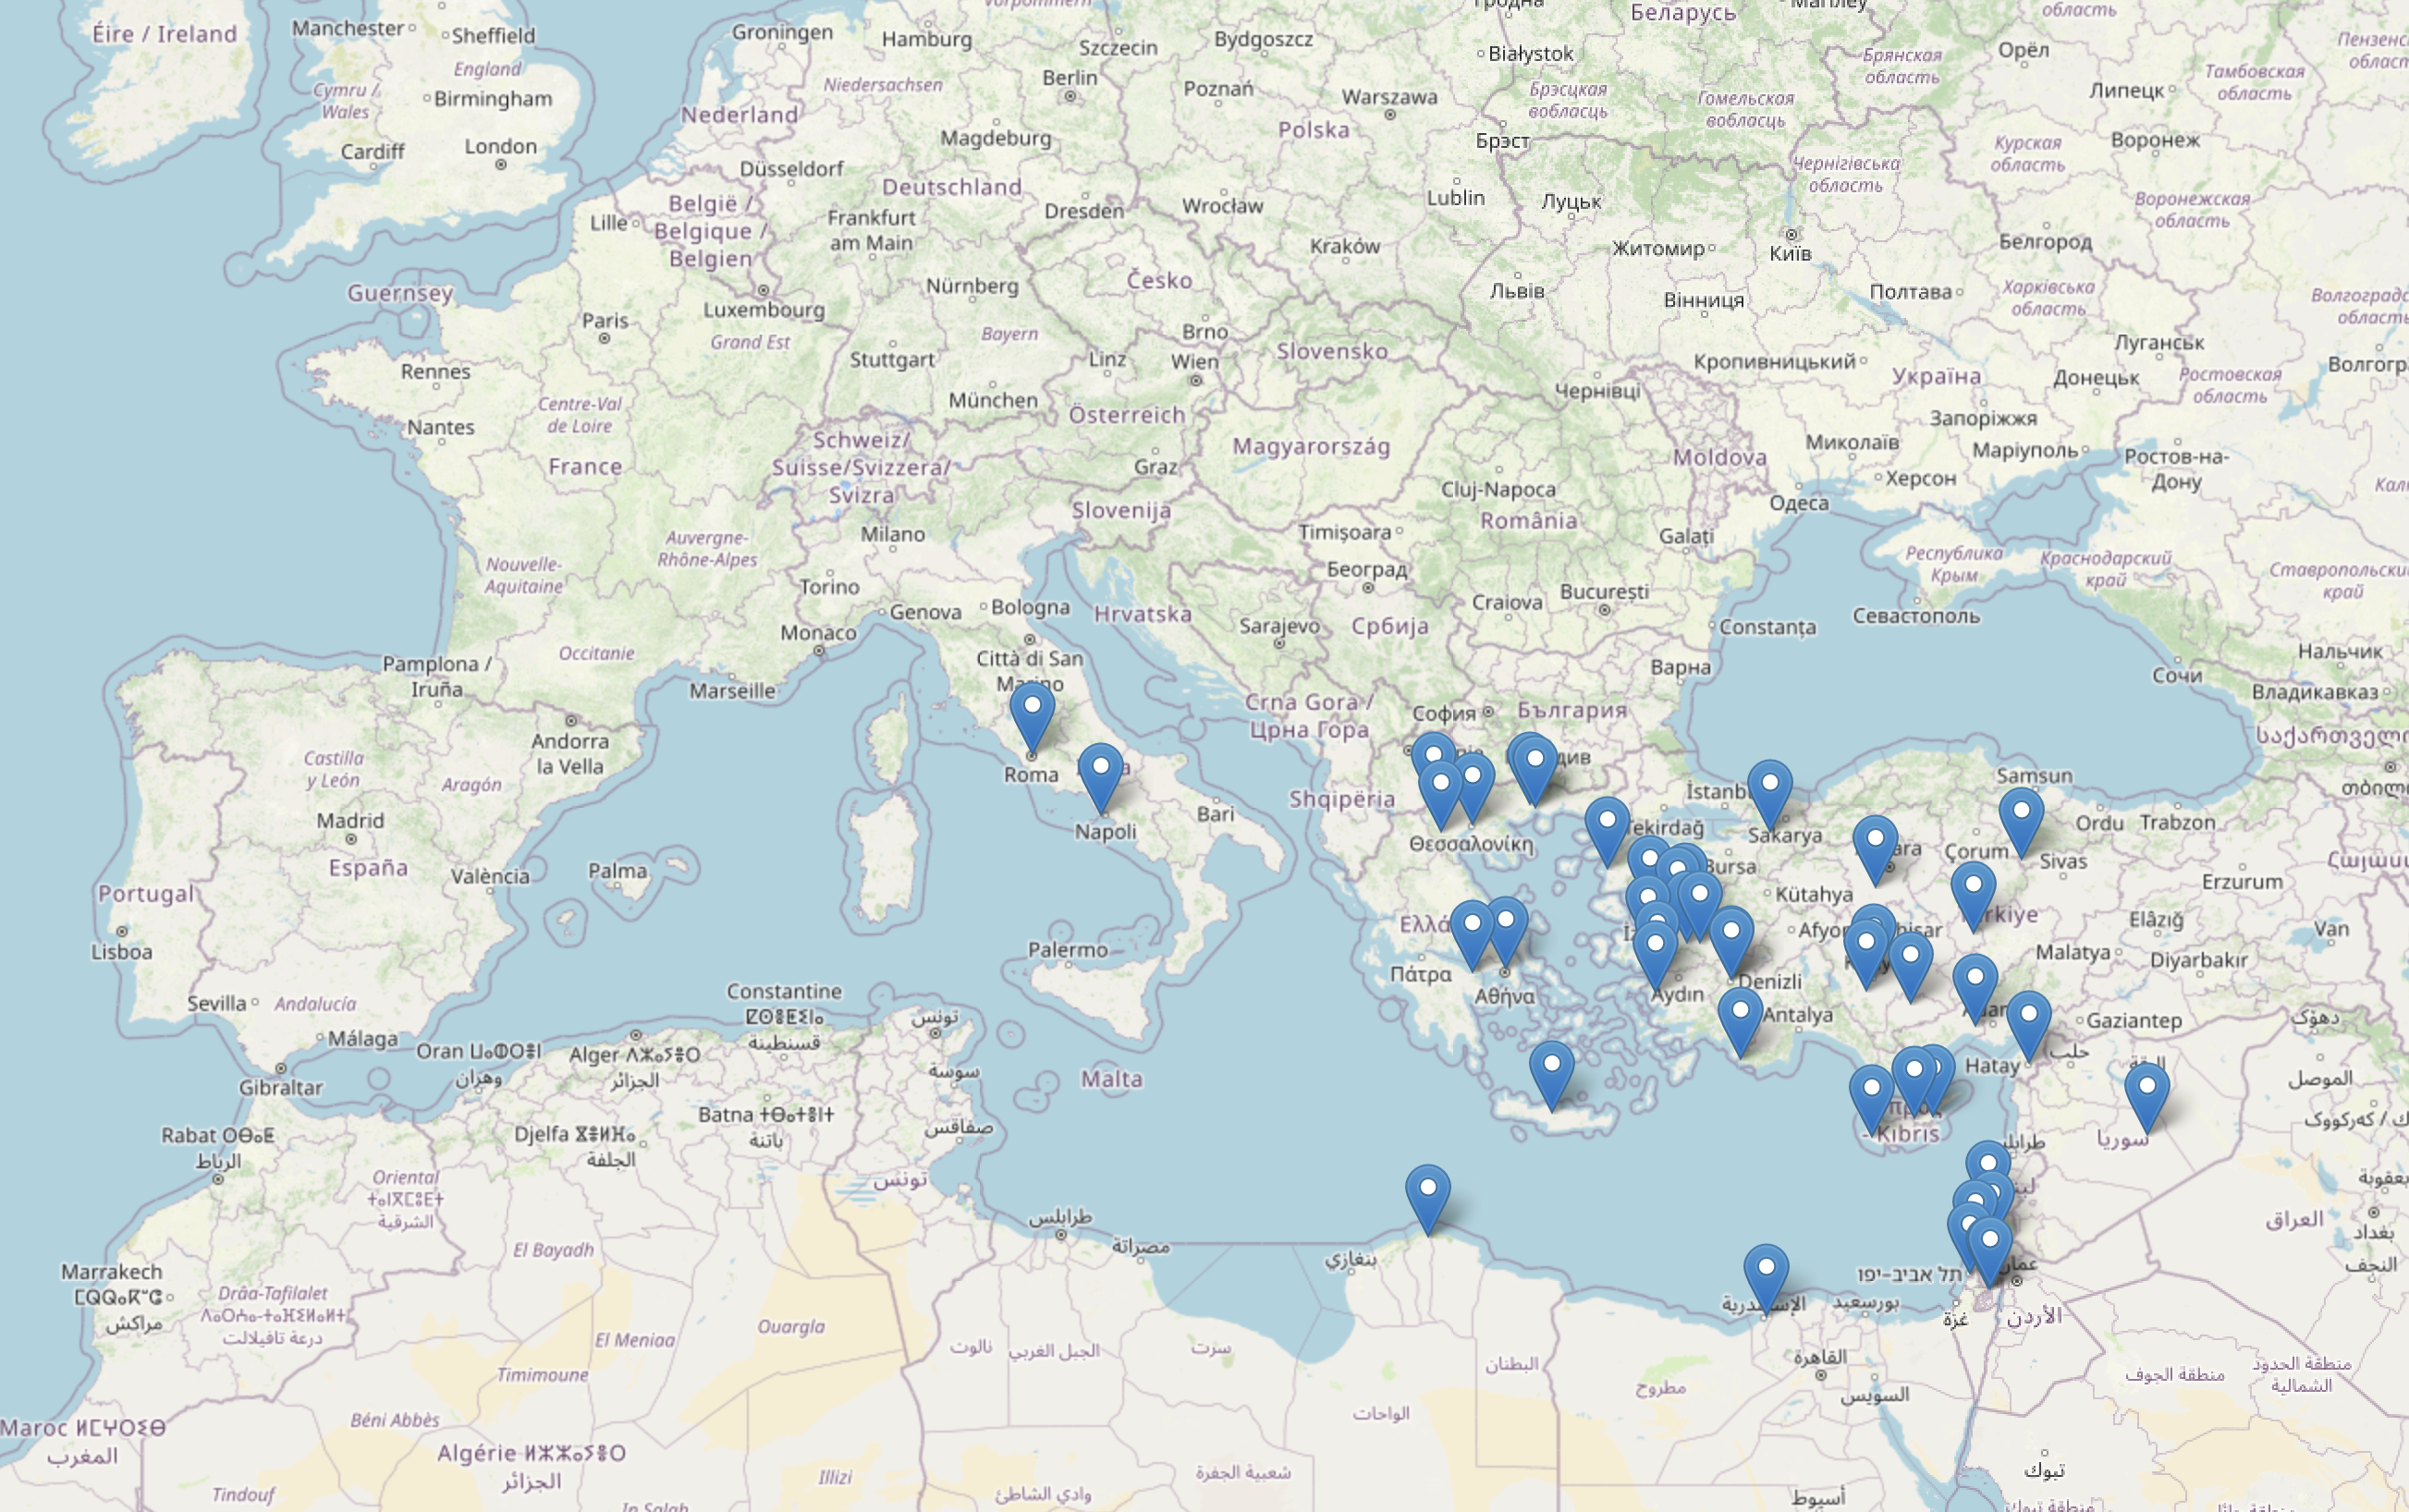
\includegraphics[width=\textwidth, keepaspectratio]{assets/locations_map}
    \caption{Map of all the locations mentioned in the Acts and the epistles.}
    \label{fig:figure}
\end{figure}

For those geographically inclined you can spot the near perfect correlation with the borders of Eastern Roman Empire.
Of note is the trip to Rome, which was substantially different in nature to the other trips.
\href{https://en.wikipedia.org/wiki/Byzantine_Empire_under_the_Theodosian_dynasty\#/media/File:4KTHEODOSIAN.png}{Rome Map}

\subsection{With the exception of Rome itself, Acts and the epistles concentrate exclusively on the former territories of Alexander's empire.}\label{subsec:the-striking-statistics-of-the-cities-mentioned-in-the-acts-and-the-epistles-are-that-they-are-all-in-the-former-greek-empire-and-not-one-mention-of-a-city-in-the-roman-empire-that-was-not-part-of-the-former-greek-empire.}

This selection rule---saturating the old Alexandrian domains while omitting Greek-speaking cities beyond those borders---makes any theory that treats Christianity as purely religious rather than political immediately implausible.

\subsection{Minimal resistance to the acceptance of the new religion.}\label{subsec:minimal-resistance-to-the-acceptance-of-the-new-religion.}

Opposition in Greek cities is framed as civic disorder, economic disruption, or public order violations---not as rejection of Christian theology as such.
The Ephesian silversmiths riot over lost business; Thessalonian authorities worry about sedition; Philippian magistrates object to public disturbance.
The only organized ideological opposition comes through Judean leadership networks.
This pattern is consistent with Christianity being a continuation of Greek imperial philosophy, which the Hellenized population already accepted.

\subsection{Even though the religion was so successful at converting the masses, it still had all the conspiratorial parts to it.}\label{subsec:even-though-the-religion-was-so-successful-at-converting-the-masses-it-still-had-all-the-conspiratorial-parts-to-it.}

Early Christians used secret symbols to identify each other, met at night, held communal meals, used coded iconography (fish, anchor, staurogram---a monogram combining the Greek letters tau and rho to represent the cross), and avoided public visibility due to political sensitivity.
The tau-rho and the later chi-rho are not accidental Christian inventions but successive stages in the reuse of an established Egyptian visual grammar.
The ankh had long expressed life, divine authority, and legitimacy through a crossed vertical form: vertical stem, horizontal bar, loop at top.
The tau-rho appears in our oldest surviving Christian manuscripts---P\textsuperscript{45}, P\textsuperscript{66}, and P\textsuperscript{75}---all from Egypt.
The tau-rho replicates this exact shape: a T-cross with the rho's loop forming a ``head,'' visually encoding a crucified figure as life-through-death.
Socrates Scholasticus reports that when Christians discovered cross-like signs at the Serapeum in 391, Egyptians read them as meaning ``life to come'' \cite[5.17]{socrates:he}---direct evidence that the ankh-cross equivalence remained active in Alexandria.
The chi-rho, which appears on Christian gems as early as the mid-third century before Constantine made it imperial, preserves the same cruciform grammar while adding explicit Christological reference.
When Christianity moved from a maThe earliest securely dated Christian manuscripts from Oxyrhynchus are overwhelmingly Johannine, establishing Egypt's earliest scriptural profile.nuscript-bound movement to an imperial regime, the same visual grammar re-emerged openly, now proclaiming sovereignty rather than encoding it.
The shape does not change; only the political visibility does.
Both Mithras and Christianity operated as discreet, oath-bound, initiatory brotherhoods---the difference is theological content, not sociological form.
The Pauline language of ``soldiers of Christ'' fits this conspiratorial military model.

\subsection{Christianity was uniquely legible to Roman authorities as a loyalty problem.}\label{subsec:christianity-much-more-prosecuted-than-any-other-religion-in-the-roman-empire.}

The Roman empire was tolerant of religions that posed no threat to imperial order.
Christians were persecuted not for worshipping a strange god, but for refusing the Roman emperor cult while insisting that only their Christ was king.

The most broadly known source of early Christian persecution, the Nero accusation of Christians starting the Great Fire of Rome, has long been disputed, with significant textual and historiographical problems noted by multiple classicists, despite its acceptance in mainstream reconstructions.
The Tacitus passage \cite[15.44]{tacitus:annals} contains the variant ``Chrestianos'' rather than ``Christianos,'' appears nowhere else in ancient literature for centuries, and describes a group Tacitus himself seems unfamiliar with, writing fifty years after the events.
Pliny the Younger, in his letter to Trajan \cite[10.96]{pliny:letters}, similarly indicates he had never participated in trials of Christians and was unsure of proper procedure.
If Christians had been publicly blamed for the largest disaster in living memory, this unfamiliarity would be difficult to explain.

At the same time, Peter was executed in Rome by crucifixion, and Paul was executed by beheading.
Like with Jesus, crucifixion was reserved for crimes against the state, sedition, and treason.
As Paul was a Roman citizen, he would have been beheaded for the same crimes.
If there was no organized persecution of Christians, it is hard to explain why both Peter and Paul were executed in such a manner.

\subsection{The phrase ``soldiers of Christ'' is not used explicitly in the Gospels, but it appears prominently in the Pauline Epistles.}\label{subsec:the-phrase-soldiers-of-christ-is-not-used-explicitly-in-the-gospels-but-it-appears-prominently-in-the-pauline-epistles-particularly-in-the-context-of-the-christian-life-being-compared-to-a-military-struggle-or-a-spiritual-battle.}

In the Roman world, military metaphors were never just metaphors.
Roman writers used soldier-language for groups that took oaths, had secret loyalties, maintained internal discipline, and operated in cells or brotherhoods.
Cicero calls Catiline's conspirators ``soldiers of Catiline'' long after they were unarmed \cite[2.5]{cicero:catilinam}.
Josephus describes followers of Judas the Galilean as ``disciplined like soldiers'' even though they were not a formal army \cite[18.23]{josephus:ant}.
Plutarch describes political factions as acting ``like soldiers,'' even without weapons \cite[Life of Sertorius 26]{plutarch:lives}.
Whenever a movement was oath-bound or aimed at regime change, Roman authors defaulted to soldier-language even when no open army existed.

Paul uses this vocabulary extensively: στρατιώτης Χριστοῦ, ``soldier of Christ'' (2 Tim 2:3); συστρατιώτης, ``fellow-soldier'' (Phil 2:25; Phlm 2); στρατεία, ``military campaign'' (1 Cor 9:7; 2 Cor 10:3--4); πανοπλία, ``full armor'' (Eph 6:11).
All four terms belong to oath-taking, disciplined obedience, readiness for conflict, and collective struggle.
An ancient reader hearing ``soldiers of Christ'' would not hear a cute metaphor.
They would hear: this is a loyalty-group organized like an army.

Roman interrogations of Christians confirm this reading.
Pliny, Tacitus, and the \emph{Acta Scillitanorum} \cite{actascillitanorum} repeatedly accuse Christians of illicit meetings, secret oaths, refusing the imperial cult, and belonging to a \emph{collegium illicitum}.
Romans describe them as oath-bound, disciplined groups---much closer to soldier units than to voluntary worship clubs.
If Christians were openly using soldier language, Roman officials took it literally.

Paul's cities---Philippi, Corinth, Thessalonica, Ephesus, Antioch---all had permanent or semi-permanent Roman garrisons.
When Paul labels trusted companions as ``fellow-soldiers,'' he gives them the standard Roman title for cell leaders inside an organized movement.
This makes full sense in a world where Jesus is king, the kingdom is real, loyalty to Christ conflicts with loyalty to Caesar, and believers act like an underground structure preparing for political realignment.

\section{The early dating of the gospels can make the letters of Paul more plausible as it seems Paul already has the knowledge of at least one of the gospels and the acts.}\label{sec:the-early-dating-of-the-gospels-can-make-the-letters-of-paul-more-plausible-as-it-seems-paul-already-has-the-knowledge-of-at-least-one-of-the-gospels-and-the-acts.}

Scholars dispute the authenticity, composition process, and dating of specific Pauline letters, noting that the authors of some epistles seem to presuppose knowledge of the gospels and Acts, even though these texts are conventionally dated after the Pauline corpus.
This tension dissolves if we acknowledge the early dating of the gospels and the gospel of John as written by an eyewitness of Jesus's life.

\subsection{Paul barely mentions the life of Jesus, and almost never quotes him.}\label{subsec:paul-barely-mentions-the-life-of-jesus-and-almost-never-quotes-him.}

It is frequently claimed that Paul's religion is not the religion of Jesus, but the religion about Jesus.
There is a shocking lack of references to any of the teachings of Jesus, the Jewish law, and any of the events surrounding Jesus's life and death.
So we may go one step further.
It is a religion focusing on restoring the kingdom of God by resurrecting the office of the Christos, the rightful king of the kingdom of God.
And so to Paul and all the early Christians, it was all about resurrecting a Christ, not teachings of the particular Jesus Christ.
The idea that God will once again send a king that will restore the Greek empire, the kingdom of God, headed by Christos, the rightful earthly king of the kingdom of God.

\subsection{Using this conspiratorial language clearly worked.}\label{subsec:using-this-conspiratorial-language-clearly-worked}

Rome did not even realize the new religion's goal was to restore the Eastern Empire until it actually happened.

\subsection{10.
Alexandria was the capital of the Greek Empire and the center of the Hellenistic world and yet there are no missions or letters to Alexandria.}\label{subsec:alexandria-was-the-capital-of-the-greek-empire-and-the-center-of-the-hellenistic-world-and-yet-there-are-no-missions-or-letters-to-alexandria.}

The absence of Alexandria in the New Testament is striking, especially considering its significance.
Alexandria hosted the largest Jewish community outside Palestine, the only city where Jewish population rivaled Jerusalem itself.
The city produced the Septuagint, the Wisdom literature, Philo's philosophical corpus, and the conceptual vocabulary that fills the Gospel of John.
Yet no epistle addresses Alexandria; no mission narrative targets it.
This silence follows the same pattern visible in the other apostolic spheres.
An apostle writes from his metropolitan center to his mission field, not to his point of origin.
James does not write to Jerusalem; Peter does not write to Antioch; Paul does not write to Ephesus as mission target.
One plausible explanation is that Alexandria functioned as a point of origin rather than a mission field, which would explain its absence from apostolic correspondence; this is consistent with the early Egyptian papyrological and reception evidence for Johannine material, even though later traditions relocate John to Ephesus.
The city appears only obliquely, as the origin of Apollos (Acts 18:24), who arrives already trained in the Scriptures and requiring only correction on baptism.
This is not the profile of a new convert but of someone formed in an already-established Alexandrian community.
The omission is best explained as deliberate suppression, precisely because Alexandria was already the center of the movement.
Just as the Old Testament largely omits the Ptolemaic empire despite its centrality, so the New Testament minimizes Alexandria while presuming its leadership.

\section{Acts of the Apostles}\label{subsec:acts-of-the-apostles}

Some scholars classify Acts of the Apostles as ancient fiction or novel.
Acts repeatedly names precise civic offices confirmed by inscriptions, including politarchs in Thessalonica, Asiarchs in Ephesus, and a proconsul in Cyprus, titles unknown or misused by later forgers.
The narrative tracks legal procedures, assembly competences, travel routes, ports, and intercity logistics with administrative precision that exceeds the needs and habits of fiction.
The so-called ``we'' passages function as itinerary notes embedded in the narrative, not as literary devices of characterization or drama.
Acts records treasuries, letters of recommendation, jurisdictional disputes, and debates over common law between assemblies, all of which are institutional details fiction does not require.
A fictional novel has no incentive to burden itself with this volume of verifiable administrative exactitude.
Acts of the Apostles is not biography, not myth, and not a religious tract.
Acts shares notable features with pragmatic Greco-Roman historiography concerned with power, legitimacy, and regime formation, inviting comparison with authors such as Polybius \cite{polybius:histories}, who writes history to explain how sovereignties rise, stabilize, and confront rivals, rather than Plutarch, who writes moral lives.
Luke's preface (Luke 1:1--4) follows formal historiographic conventions of orderly narration, eyewitness sourcing, and public verification.
Throughout Acts, βασιλεία denotes real sovereignty and jurisdiction, not interior spirituality or ethical sentiment.
Acts 1:6 frames the narrative program explicitly as the restoration of a kingdom, not the founding of a cult.
That question presupposes a Hellenistic world of competing regimes rather than a private religion.
Acts narrates the collision between a renewed kingdom claim and existing imperial powers across the Greek world.
The final scene places Paul in Rome proclaiming ``the kingdom of God,'' which functions as a regime proclamation at the imperial center.
The book closes not with conversion stories but with an unresolved contest of sovereignties.

\subsection{10.
Acts opens with a royal enthronement}\label{subsec:acts-opens-with-a-royal-enthronement}

Acts 1:6 --- ``Lord, will you at this time restore the kingdom to Israel?'' This is not a spiritual question.
It implies Jesus had a claim to political kingship.
Your theory: Jesus was understood as the rightful monarch of a revived kingdom---a successor to the Herodian or Hasmonean thrones under Greek imperial ideals.

\subsection{10.
Jesus is taken up like an emperor}\label{subsec:jesus-is-taken-up-like-an-emperor}

Acts 1:9--11 --- The Ascension mimics apotheosis scenes (e.g., Alexander, Roman emperors).
It frames Jesus in imperial terms, being enthroned in heaven---like a divine emperor.
This matches your view that Christianity was about loyalty to the ``Christ Emperor.''

\subsection{10.
The Pentecost scene mimics an imperial inauguration}\label{subsec:the-pentecost-scene-mimics-an-imperial-inauguration}

Acts 2 --- Multilingual miracle and mass conversion reflects the imperial ideal of uniting nations under one divine king.
The language of ``tongues'' is political: the emperor's message is for all nations.

\subsection{10.
Acts 5: The trial of the apostles}\label{subsec:acts-5-the-trial-of-the-apostles}

Gamaliel references past revolutionary figures---Theudas and Judas the Galilean.
This acknowledges that messianic revolts were political, and that Jesus' movement was seen in similar terms.

\subsection{10.
Stephen's speech in Acts 7 is anti-Temple}\label{subsec:stephens-speech-in-acts-7-is-anti-temple}

Stephen attacks the Temple and Mosaic tradition, echoing Philo and Stoic-influenced criticisms of Jewish legalism.
This supports the view that early Christianity rejected the Mosaic religion and aligned more with philosophical monotheism.

\subsection{10.
Acts ends without resolution}\label{subsec:acts-ends-without-resolution}

The book ends in Rome, with Paul freely preaching ``the kingdom of God.''
It lacks a narrative climax because its real message is that the empire is now Christian.
It presumes a pre-existing audience that sees Christianity as a political-theological force.

\subsubsection{James the Just}\label{subsec:james-the-just}

\subsection{James the Just also wrote an epistle to all nations.}\label{subsec:james-the-just-also-wrote-an-epistle-to-all-nations.}

He was the brother of Jesus, and within the dynastic framework of this book, the next in line to the throne.
This book argues that honorifics such as ``the Just'' function within the same Hellenistic titulature system as Soter or Epiphanes, and should be read accordingly.

James the Just also wrote an epistle to all nations, which is included in the New Testament.
The rhetorical style of James---moral diatribe with imaginary interlocutors, imperatival exhortation, vivid examples---belongs to the same Hellenistic tradition of philosophical moral teaching that Philo inherited.
James shares the moral-philosophical register of Hellenistic paraenesis more than any distinctively Jewish sectarian idiom.

In Greek, James 1:21 reads as:
``Διὸ ἀποθέμενοι πάσαν ἀκαθαρσίαν καὶ περισσείαν κακίας ἐν πραΰτητι δέξασθε τὸν ἐμφυτον λόγον, ὃς δύναται σῶσαι τὰς ψυχὰς ὑμῶν.''
Transliteration: ``Dio apothemenoi pasan akatharsian kai perisseian kakias en prautēti dexasthē ton emphuton logon, hos dynatai sōsai tas psychas hymōn.''
A literal translation: ``Therefore, putting away all filthiness and the overflow of wickedness, with meekness receive the implanted word, which is able to save your souls.''

The Epistle of James is written in polished literary Koine, using complex subordination, a broad and partly creative vocabulary (with over sixty words unique in the New Testament), and the rhetorical techniques of Hellenistic moral diatribe---paronomasia, alliteration, personification, and vivid rhetorical questions.
This level of Greek is difficult to reconcile with an illiterate village laborer and points instead to a figure embedded in the educated, Greek-speaking networks of the Eastern Mediterranean, whether by personal training or by collaboration with a skilled scribe.

\subsubsection{The Epistles of John}\label{subsec:the-epistles-of-john}

\subsection{A disproof of existing models}\label{subsec:a-disproof-of-existing-models}

The scholarly literature usually explains the rise of Christianity through one of three frameworks: the missionary diffusion model, the Judaic sect model, or the imperial cult competition model.
All three assume Christianity began as a small religious group and gradually expanded through organic processes.
The actual data show this assumption is impossible.

\textbf{1. Missionary Diffusion Model (Harnack, Stark, etc.).}
This model imagines apostles traveling city by city, converting households, and founding local congregations which then grew over time.
It predicts: (a) gradual spread across regions, (b) uneven adoption, (c) multilingual documentation, and (d) continuous growth into the second century.
\emph{Observed:} a sudden network of churches in every major polis of the Greek East, exclusively in Greek, followed by a century of stagnation.
\emph{Conclusion:} the model cannot account for this. Gradual spread does not yield instantaneous empire-wide presence and then silence.

\textbf{2. Judaic Sect Model (Eisenman, Sanders, Vermes, etc.).}
This model portrays Christianity as a messianic reform within Judaism that later opened to Gentiles.
It predicts: (a) early writings in Aramaic or Hebrew, (b) reliance on Mosaic law and Temple tradition, (c) expansion via diaspora synagogues, and (d) later translation into Greek.
\emph{Observed:} not a single Aramaic or Hebrew letter, no synagogue-based diffusion, hostility to Mosaic law, and universal Greek correspondence.
\emph{Conclusion:} the expected Jewish framework is entirely absent. The movement is Greek and imperial from its inception.

\textbf{3. Imperial Cult Competition Model (Friesen, Harland, etc.).}
This model treats Christianity as another civic cult competing in the Roman religious marketplace.
It predicts: (a) incremental adoption across both Latin West and Greek East, (b) local diversity of practice, (c) syncretism with Roman emperor worship, and (d) gradual growth from private associations to public cult.
\emph{Observed:} no spread into the Latin West, no random scatter across Roman cities, but perfect coverage of the former Greek empire with uniform claims of one royal Christ.
\emph{Conclusion:} the data negate this model. Instead of scattered cult competition, the pattern is coherent and centralized.

\textbf{Final judgment.}
Every alternative model collapses.
Their predictions do not merely “fit poorly” --- they are completely impossible to reconcile with the actual evidence.
It is therefore certain that early Christianity was not the product of missionary growth, sectarian Judaism, or cult competition.
The churches were not newly founded congregations but the continuing \textit{ekklesiai} of the Greek world, reorganized under Christos.
The sequence of events --- zero presence, immediate imperial coverage, then long stagnation --- admits only one explanation: continuation of the Greek empire under a new royal proclamation.

\subsection{The Corpus of the New Testament}\label{subsec:the-corpus-of-the-new-testament}

What is actually in the New Testament, and how does it map onto the four imperial poles we have identified?
Below we make the mapping explicit \emph{and} anchor it with specific ancient evidence, especially for the epistles and early authorship claims.
Note well: in antiquity the attributions of the four canonical gospels to \textit{Matthew, Mark, Luke, John} are uniformly asserted by the Fathers.
No alternative apostolic names are recorded for them.

\subsection{Patristic attestations (authorship in antiquity).}
Before the mid-third century the picture is consistent.
\textbf{Papias} (via Eusebius \cite[3.39]{eusebius:he}) --- Mark wrote as Peter's interpreter.
Matthew compiled the \textit{logia}.
\textbf{Irenaeus} \cite[3.1.1]{irenaeus:advhaer} --- explicitly lists and defends the four: Matthew, Mark, Luke (Paul's companion), John.
The \textbf{Muratorian Fragment} (late 2nd c.) names Luke and John as the third and fourth gospels and recognizes a Pauline corpus.
\textbf{Clement of Alexandria} \cite{clement:stromata} and \textbf{Origen} \cite{origen:contracels} repeat these attributions.
\textbf{Eusebius} later summarizes them as received.
For epistles: \textbf{1~Clement} (c.~96) cites 1~Corinthians.
\textbf{Ignatius} (c.~110) presupposes Pauline churches and diction.
\textbf{Polycarp} (c.~135) quotes or echoes multiple Pauline letters and 1~Peter.
\textbf{Irenaeus} uses 1--2~Peter, 1~John, and James as apostolic.
Discussion about Hebrews’ author and the lateness of 2~Peter appears later.
Crucially, there is no early counter-attribution of the \emph{four gospels} to other names.

\subsection{Papyri and early circulation (snapshot).}\label{subsec:papyri-and-early-circulation}
\textbf{P\textsuperscript{46}} (c.~200) preserves a Pauline collection (Rom, 1--2~Cor, Gal, Eph/Col, Phil, 1~Thess, Heb), showing the letters already circulated as a corpus.
\textbf{P\textsuperscript{66}} (c.~200) and \textbf{P\textsuperscript{75}} (early 3rd c.) are major early witnesses to John (and Luke/John).
\textbf{P\textsuperscript{9}} (3rd c.) preserves 1~John at Oxyrhynchus.
\textbf{P\textsuperscript{72}} (3rd/4th c.) contains 1--2~Peter and Jude.
\textbf{P\textsuperscript{13}} (3rd c.) Hebrews.
\textbf{P\textsuperscript{45}} (3rd c.) Gospels/Acts.
These confirm early circulation and natural clustering (Pauline set; Petrine/Jude; Johannine) that mirrors our four-pole architecture.
Egyptian findspots reflect preservation bias.
The \emph{composition} clustering still tracks the imperial map.

\subsection{The Four Surviving Greek Cultural Worlds After Alexander}

The existence of four canonical gospels was not a later editorial accident or a theological compromise.
It reflects something far older and deeper: the Eastern Mediterranean itself was structured into four great cultural worlds that had survived intact since the breakup of Alexander's empire.
The gospels emerged inside that fourfold world, and their differences mirror those four surviving Greek cultural spheres.

When Alexander's empire disintegrated, it did not splinter into dozens of equal states; it crystallized almost immediately into four dominant dynastic regions, each of which became a self-contained cultural ecosystem with its own institutions, its own Greek idiom, and its own political memory.
These were not merely kingdoms in a political sense; they were civilizational spheres, each large enough to shape millions of people and stable enough to endure for centuries, even after their kings vanished.
Every major city, people, and educational system in the Eastern Mediterranean belonged to one of these four worlds.

Ptolemaic Egypt built the most intellectually ambitious Greek culture of the ancient world.
Alexandria remained the uncontested center of scholarship, Jewish--Greek philosophical synthesis, textual production, and metaphysical speculation, even after Augustus annexed Egypt.
Its institutions outlived the dynasty: the Museum, the philosophical academies, the scribal culture, and the distinctively Alexandrian style of conceptual Greek all survived intact.
This is the world that produced the Logos theology, Platonic dualisms, revelatory dialogues, and metaphysical vocabulary that characterize the Gospel of John.
John is not an anomaly; he is the voice of Alexandrian Judaism speaking Greek in its own intellectual register.

Seleucid Syria, with Antioch as its capital, developed a completely different Greek environment: a Greek metropolis set at the edge of an Aramaic-speaking countryside.
This region's linguistic reality was stable and unmistakable---Greek in the cities, Aramaic in the hinterland---which produced a natural, effortless bilingualism.
Short imperatives, nicknames, exclamations, healing commands, and frontier expressions migrated constantly between languages.
This is exactly the pattern preserved in Mark's Aramaic phrases.
These are not the relics of a Galilean Jesus; they are the code-switching habits of an Antiochene Greek author writing inside a Syrian--Seleucid bilingual world.
The frontier heroic style, the abrupt narrative, the epic-mimetic structure, and the mixture of Greek and Aramaic all fit Antioch perfectly and Galilee not at all.

The Judean kingdom, created by the Hasmoneans long before Rome entered the region, was the project of a large, coherent, politically ambitious people determined to govern themselves.
They were not a Roman creation.
They seized independence because, at the collapse of Seleucid power, they were strong enough and organized enough to form their own dynasty and maintain their own traditions inside the Greek oikoumene.
The Herodian successors continued this world in a different key, but the cultural bloc persisted: a region with its own law schools, its own dynastic memory, its own debates about legitimacy, and its own identity within Greek political culture.
The Gospel of Matthew reflects this environment precisely: dynastic genealogy, legal-exegetical argument, fulfillment formulas, and a Judean political theology expressed in Greek, not the Aegean rhetorical style or the Alexandrian metaphysical style or the Syrian bilingual style.

The Antigonid world---Macedonia, Greece, and the Aegean basin---was the fourth great post-Alexandrian culture.
Even after the Antigonid dynasty itself was crushed, the institutions it built endured unchanged.
The gymnasia, the classical rhetoric schools, the polis assemblies, the honorific decrees, the elite historiographic tradition, and the educational system of the Greek mainland and western Asia Minor all descended from Antigonid foundations.
By the first century, Ephesus had emerged as the de facto metropolis of this entire region: the largest, wealthiest, most institutionally Greek city of the Aegean world.
This is the cultural sphere that produced Thessalonica, Philippi, Corinth, and the wider Pauline urban network.
It is also the sphere reflected in Luke's Greek: the polished historiographic proem, the administrative precision, the nautical vocabulary, the civic terminology, and the rhetorical structure taught in Aegean gymnasia.
Luke is not writing generic Greek; he is writing the Greek of the classical educational capital of the Mediterranean.

These four worlds were the only meaningful large-scale cultural divisions of the Greek East.
Every other division is artificial.
Every region fell under one of these blocs.
Their institutional cultures survived long after the dynasties ceased to rule.
Under Roman administration these four worlds still existed as cultural facts: Alexandria still thought like the Ptolemies, Antioch like the Seleucids, Jerusalem like its native dynasty, and the Aegean cities like the Antigonid world.

This is why the diversity of the gospels finally makes historical sense.
Each gospel is not just a theological portrait; it is the product of one of these four great cultural ecosystems.
John speaks from Alexandria.
Mark speaks from Antioch.
Matthew speaks from Judea.
Luke speaks from the Aegean world.
The fourfold gospel is not an accident of canon formation; it is the literary map of the four surviving Greek cultures of the Eastern Mediterranean.
But the fourfold structure itself is older than Alexander.

\subsection{The Four Royal Symbols Before Alexander}

The fourfold map that shapes the gospels was not invented in the Hellenistic age.
Readers will immediately notice that Ezekiel prophesied in the sixth century BC, long before Alexander's empire fractured into Ptolemies, Seleucids, Hasmoneans, and Antigonids.
This chronological distance is not a problem; it is the key.
Ezekiel's vision belongs to a world where the Near East had already used four royal symbols for over a thousand years.
These symbols were not decorative.
They were the official state insignia, military standards, temple icons, and royal emblems of the four great cultural spheres that predated all later empires.
When Ezekiel sees a lion, a bull, a \emph{nešer}, and a human, he is describing the established political and cosmological grammar of the ancient Near East---the way kingdoms represented power.
The Hebrew \emph{nešer} (נֶשֶׁר) does not denote a zoologically precise ``eagle'' but a royal bird of prey in a high-register iconographic sense; in Ezekiel's context it can plausibly encompass falcon imagery and is fully compatible with the Horus falcon symbolism dominant in sixth-century BC Egypt.
These four emblems stand at the core of the region's political theology long before the gospels and long before Hellenistic rule.

For more than two thousand years before Ezekiel, Egypt's symbol of kingship was the crowned falcon of Horus, perched above the royal name in every cartouche.
Every pharaoh from the Old Kingdom onward was explicitly styled ``Horus,'' and the falcon-bird was placed on standards, palace façades, funerary temples, military banners, and royal jewelry.
By the Late Period---Ezekiel's own lifetime---the falcon remained the official emblem of Egyptian sovereignty, appearing on throne iconography, priestly regalia, and monumental reliefs.
This is why Ezekiel's \emph{nešer} face is instantly recognizable: he invokes the eastern symbol of divine kingship, the creature that literally sits on the head of every Pharaoh as the uraeus--Horus pairing.
When the Ptolemies later rule Egypt, they adopt the Eagle of Zeus, which is simply the Greek equivalent of the Horus-falcon: the royal sky-bird, the emblem of sovereignty.
This symbol is so dominant that it becomes the Roman legionary eagle, and through Rome becomes the emblem of the Byzantines, Germans, Russians, Poles, Americans, and the Arab republics.
The eagle is the oldest continuous royal symbol of the eastern Mediterranean and the political face of the eastern quadrant of the ancient world.

In the western Levant---the Phoenician and Aramaean world---the bull was the supreme symbol of state authority for at least a thousand years before Alexander.
The bull was the living emblem of Baal and Hadad, the region's royal storm-god, who sits enthroned upon a bull in Ugaritic tablets of the thirteenth and twelfth centuries BC, controls rain, and legitimizes kings.
Phoenician temples from Byblos, Tyre, and Sidon displayed bronze bulls at their gates; Aramaean cities carved bull-statues as guardian figures; and royal seals across Canaan show bull-headed deities conferring authority on kings.
When the Bible describes Israel building a golden calf, it is not describing a random idol---it is describing the official Phoenician state god, the royal emblem of the entire coastal monarchy system.
By the time of Ezekiel, the bull is already the recognized symbol of the western quadrant, the agricultural and maritime world ruled by storm-gods.
When the Seleucids later build their empire on this same region, they adopt a hybrid of bull, horse, and horned power imagery that continues this millennia-old emblem of authority.
Ezekiel's ox face is therefore not an animal chosen at random; it is the political symbol of the whole western Levantine--Syrian bloc.

Long before Ezekiel, the lion had already become the canonical emblem of kingship across the West-Semitic interior, from Canaan and Moab to Israel and Judah.
Assyrian palaces carved endless lion-hunt reliefs because the lion symbolized royal dominance, and Babylon erected entire avenues of lions for state ritual.
The biblical ``Lion of Judah'' is not a cute metaphor: it is the Judean state emblem attested in royal ideology since at least the time of David, reinforced in the blessing of Judah in Genesis 49, and supported by lion-imagery on Judean seals, storage jars, and monumental architecture.
The lion's power over the desert, its predatory ferocity, and its association with royal conquest made it the natural symbol of the southern quadrant: the West-Semitic highlands and frontier deserts.
In Ezekiel's world the lion already functions as the identity-marker of Israel's royal lineage, just as the falcon identifies Egypt and the bull identifies Phoenicia.
Ezekiel's lion face therefore stands for the southern royal culture of the Near Eastern symbolic map.

The fourth symbol---the human---is not meant to be weak or neutral.
It is the heroic human, the figure that dominates Greek art from the Bronze Age onward.
Mycenaean frescoes and kraters show helmeted warriors; Geometric-period pottery shows hoplite ranks; Archaic sculpture develops the kouros as the ideal military citizen; and Classical Athens, Sparta, and Macedon use the armed human figure as their primary emblem of civic identity.
The Greek world is the only Near Eastern cultural bloc whose sovereign symbol is explicitly anthropic: Achilles, Ajax, Heracles, Perseus, Theseus, and ultimately the hoplite citizen.
For at least seven centuries before Ezekiel, the Aegean world's political theology is built around the heroic man rather than an animal-god.
This is why Ezekiel's fourth face---the human---belongs to the northern quadrant, the mountains and city-states of Anatolia and Greece.
When Alexander expands Greece into an empire, he does not create this identity; he globalizes what was already the human-heroic emblem of Greek rule.

By the time Ezekiel writes in the sixth century BC, these four insignia have already dominated the region for over a millennium: the falcon for Egyptian kingship, the bull for Phoenician and Syrian authority, the lion for Judean and West-Semitic royalty, and the human hero for Anatolian and Greek warrior states.
His four-faced creature is the oldest surviving literary representation of the Near Eastern fourfold world, combining the four royal symbols, the four cultural blocs, the four winds, the four throne-bearers, and the fourfold cosmic structure.
When the early Church later says the gospel must be fourfold because the world is fourfold, they are not being mystical.
They are remembering this ancient symbolic architecture---one that predates Alexander, predates Israel's monarchy, and predates Ezekiel himself.
And when the four canonical gospels fall into the hands of Alexandria, Judea, Syria, and the Aegean, they are stepping directly into a four-quadrant world-system that had been visually and politically defined for at least a thousand years by the falcon, the bull, the lion, and the hero.

\subsection{Why Irenaeus Was Not Wrong}

The earliest Christian to explain why there are four gospels is Irenaeus, and he gives a reason almost everyone today mocks: the gospels correspond to the four living creatures---lion, ox, eagle, man---the same four beings from Ezekiel and Revelation.
Scholars dismiss this as numerology.
They treat it as mystical embroidery or primitive symbolism.
But that dismissal is completely shallow.
Irenaeus is not picking animals at random.
He is drawing on a rigid, inherited four-direction cosmology---the same symbolic architecture used in ancient apocalyptic literature---and that four-way structure is exactly how the post-Alexandrian Mediterranean world was actually divided.
His symbolic language happens to sit directly on top of a geopolitical reality.

Irenaeus was not alone.
The four-creature schema runs through the entire patristic tradition.
Revelation is the first Christian text to pick up Ezekiel's throne vision and make it central to Christian cosmology: John describes four living creatures ``in the midst of the throne and around the throne'' (Rev 4:6--8), each with a different face---lion, calf, human, eagle---chanting the Trisagion without rest, exactly as Ezekiel's cherubim marked the presence of God's glory.
Already in the New Testament, Ezekiel's fourfold creature has become part of a Christian grammar of the cosmos and the throne, not a marginal curiosity.

Scholars have long agreed that Revelation's Beast is not an abstract monster but a concrete ruler and regime.
The number 666 transparently encodes Nero through Hebrew gematria of Νέρων Καῖσαρ, while the 616 variant reflects the Latin spelling of the same name.
The Beast's wounds, blasphemies, persecution, and imperial cult all fit Nero precisely, and the text itself invites calculation rather than allegory.
Likewise, Babylon is not a mystical cipher but the city of Rome, identified by its seven hills and its rule over the kings of the earth.
On this reading, Revelation is not a timeless drama of good and evil but a focused apocalyptic announcement of Rome's judgment and collapse.

Yet the same scholarship that insists on this political concreteness abruptly suspends it when the vision turns from the Beast to the throne.
The four living creatures---lion, calf, human, eagle---are treated as abstract cosmic symbols or theological ornaments, detached from history and power.
This move is methodologically indefensible.
Revelation does not change its symbolic grammar halfway through the book.
The Beast is political because the symbols are political.
If Nero and Rome are real, then the throne vision is real in the same sense.

The four creatures therefore represent concrete powers aligned with God's rule, not vague metaphysical principles.
They stand in ordered opposition to Rome's Beast, just as the Kingdom of God stands in ordered opposition to Babylon.
Revelation stages a clash of empires, not a retreat into abstraction.

By the end of the second century Irenaeus makes this grammar explicit and canonical.
In \cite[3.11.8]{irenaeus:advhaer} he takes the living creatures of Revelation 4:7 and reads them as figures of the whole ``economy'' of the Son of God, then states flatly that ``the living creatures are quadriform, and the Gospel is quadriform, and the course followed by the Lord is quadriform.''
For Irenaeus the point is not a cute allegory but a necessity: the Church is spread to the four winds, the world has four zones and four principal winds, and therefore the one Christ must be witnessed in a fourfold way if the proclamation is to match the structure of creation.

Third-century writers reinforce this logic.
Origen, in his homilies on Ezekiel \cite{origen:homezek} and Luke \cite{origen:homluke}, treats the number four as intrinsic to the Gospel tradition, tying it to the four rivers of Eden, the four winds, and the four corners of the earth, and simply assumes that Ezekiel's and John's creatures provide the basic schema for how the one Christ can be presented in multiple, non-competing forms.
Victorinus of Pettau \cite[Rev 4]{victorinus:apocalypse}, the earliest surviving commentator on Revelation, is even more blunt: commenting on Revelation 4 he writes, ``The four living creatures are the four Gospels,'' and assigns each creature to one evangelist while insisting that together they surround the throne and sing the Trisagion.
By this stage the identification is fixed: whenever orthodox Christians read Revelation's throne, they saw the canonical fourfold Gospel radiating from it.

Fourth- and fifth-century Latin theology takes this over and builds orthodoxy upon it.
Augustine devotes an entire chapter in \cite[1.6]{augustine:consensu} to ``the four living creatures in the Apocalypse, which have been taken as apt figures of the four evangelists,'' accepts the identification as obvious, and only debates which creature best fits which evangelist.
For Augustine the tetramorph means that the evangelists differ and yet agree, just as four faces can belong to one throne-chariot: the structure of four is not an accident of manuscript survival but a sign that the Spirit has distributed one Christological reality into four complementary perspectives.
Jerome, in his prefaces and commentary on Matthew \cite{jerome:matthew}, standardizes the now-familiar Western assignment---man for Matthew, lion for Mark, ox for Luke, eagle for John---and welds it to his Vulgate ordering, which dominates medieval art and liturgy.
Later Latin writers like Chromatius and Rabanus Maurus simply repeat the pattern: four living creatures, four winds, four corners of the earth, four evangelists, one throne.

The key observation is that all of these authors disagree on the details of which animal matches which book but agree absolutely that there must be four and only four.
Irenaeus, Victorinus, Augustine, Jerome, and Athanasius inherit different local traditions about animal-evangelist pairings, yet none of them even considers a fifth Gospel or a reduction to one or two; the fourfoldness is treated as cosmological, not editorial.
When they appeal to Ezekiel and Revelation, they are invoking the ancient Near Eastern conviction that the world itself is four-quartered, guarded and represented by four living powers, and that the true king's throne must stand at the center of this quadriform order.
The canonical fourfold Gospel is justified along exactly those lines: the Christ who sits between the cherubim (Ps 80:1) and in the midst of the four living creatures (Rev 4:6) must be proclaimed in four converging voices if the proclamation is to match the architecture of creation.

Modern scholarship tends to quote Irenaeus's line about four winds and four corners with a smirk, as if this were a primitive rationalization pasted onto an already fixed canon, but the patristic evidence runs the other way: the four-creature throne, the fourfold world, and the fourfold Gospel are treated as a single integrated pattern by nearly every major architect of orthodoxy.
What the church fathers lack is not symbolic intelligence but geopolitical hindsight.
They sense that the Christ-story must radiate from four faces into the whole inhabited world, and they use Ezekiel and Revelation to say so, but they do not yet name the concrete cultural blocs---Alexandrian Egypt, Judea, Syrian--Seleucid Antioch, and the Aegean Greek cities---that actually supplied those faces.
Their constant appeal to the tetramorph is therefore not a clumsy afterthought but a preserved fragment of a much older fourfold logic, one that turns out to align exactly with the real political and linguistic structure of the post-Alexandrian eastern Mediterranean once we restore that context to view.

Because the stunning historical fact is this: the four creatures they name are the four state emblems of the four great dynastic cultures that ruled the Greek East---the same four cultures that produced the four canonical gospels.

Ptolemaic Egypt did not use the eagle as decoration; it used the Eagle of Zeus as the central badge of royal power.
Every major Ptolemaic coin type---silver, gold, and bronze---shows the same unmistakable image: the Zeus-eagle standing on the thunderbolt, the most repetitive dynastic emblem in the Hellenistic world.
The same eagle appeared on Ptolemaic military standards, naval ensigns, palace iconography, and border-garrison insignia, saturating public space so completely that subjects from Cyprus to Phoenicia recognized the eagle as the visual signature of Ptolemaic authority.
The symbol did not vanish with the dynasty.
Rome adopted the very same bird as the Eagle of Jupiter, the legionary aquila, turning the Zeus-eagle into the supreme emblem of imperial power for the next five centuries.
Through Rome the emblem passed into European heraldry, becoming the imperial eagle of the Holy Roman Empire and eventually the national symbols of Germany, Poland, and---by conscious republican imitation of Roman iconography---the United States.
And in the Near East the single-headed eagle survived independently through earlier Ptolemaic saturation of Egypt and the Syrian coast, which is why modern Egypt, Syria, Iraq, Palestine, and Yemen still use the same eagle today.
The Ptolemaic Eagle of Zeus is thus one of the longest-lived state symbols in world history, and it defines precisely the cultural universe behind the Alexandrian Gospel of John.

The Seleucid emblem was established at the very top, by the founder himself.
Seleucus I Nicator struck royal gold and silver showing Bucephalus with ox-horns, a deliberate visual statement merging Alexander's legendary war-horse with the ancient bull-power of Syria.
The inscription ΒΑΣΙΛΕΩΣ ΣΕΛΕΥΚΟΥ confirms this as an official dynastic issue: the horned horse's head is the personal badge of the first Seleucid king, the stamp of legitimacy he used as he carved out his empire from Babylon to Antioch.
Once the founder fixed the symbol, the dynasty did not abandon it.
The Seleucids repeatedly used bulls, horned bulls, butting bulls, and bull-gods on their coinage for two centuries---SC 130--133, 379, 505--525, 841--856, and 1420--1421---extending the founder's horned-Bucephalus imagery into a broader bull-power system that became the visual grammar of Seleucid rule.
This is the political world behind Mark: the Syrian--Seleucid frontier where Greek kingship fused with the thousand-year bull tradition of the Levant, and where the ox quadrant of Ezekiel was not metaphor but lived reality.

The lion was the emblem of the Hasmonean and Herodian kingdom, the lion of Judah, carved into fortress stones, stamped on royal seals, carried on banners, associated with kingship and Jerusalem.
It was so central to Judean identity that the symbol survived long after the dynasty died: Ethiopia's imperial flag carried the Lion of Judah until the twentieth century.
The lion of Judah is still the emblem of the city of Jerusalem today.
Nobody in antiquity needed to be told what a lion meant in the eastern Mediterranean: it meant Judea, dynasty, legitimacy, royal memory.
This is exactly the world Matthew stands in: the dynastic, legal, succession-driven Judean tradition.

And the human warrior---the helmeted Macedonian hoplite---was the emblem of the Antigonid Aegean world.
It is the most recognizable symbol of ancient Greece to this day: the crested Corinthian helmet, the forward-facing hoplite profile, the human face of the Greek polis.
The Antigonids built the institutions of the classical Greek world---gymnasia, rhetoric schools, civic education---and their public identity was overwhelmingly human rather than animal.
This is the world of Luke---the only gospel written in the polished historiographic, civic, administrative Greek of the Aegean cities.

The phrase ``Son of Man'' belongs to this same Aegean political grammar.
In Greek political language, ἄνθρωπος functions as a representative or corporate figure: the ruler who embodies the city.
Macedonian and Antigonid kings are not divine by birth; they are men who rule well and only later receive cult.
The king is the man raised above men, not the god descended among them.
This contrasts sharply with Egyptian royal theology, where the pharaoh is divine from conception.
Greek literature routinely contrasts θηρίον (beast, tyrant, barbarian power) with ἄνθρωπος (lawful ruler).
Daniel 7's vision of ``one like a son of man'' receiving authority from the Ancient of Days translates directly into this framework: a human-type ruler contrasted with the beast-empires that precede him.
Jesus deploys the title in exactly this Aegean sense---judge of nations, receiver of authority, one who comes publicly with power---not as a Hebrew idiom for mortal frailty.
The Romans execute him as a king, not as a prophet, because they hear the political claim correctly.
Acts 16:9 records Paul's decisive redirection westward through a vision in which ``a man of Macedonia'' (ἀνὴρ Μακεδών) summons him, explicitly personifying the Aegean Greek world as a ``man.''
This vision does not depict an abstract individual but a regional political body, identifying Macedonia itself as the human counterpart to beastly empires.
The Macedonian ``man'' thus corresponds to the human figure in the throne tetramorph, anchoring the Man quadrant in Aegean political reality.
In Ephesians 3:5, Paul states that the mystery was not made known to ``the sons of men'' (τοῖς υἱοῖς τῶν ἀνθρώπων) in earlier generations.
In context, this phrase refers to Paul's specific audience within the Greek-speaking Aegean world rather than to generic humanity.
Standard readings that reduce ``Son of Man'' to a Danielic messianic title or a Hebrew idiom for mortality flatten the term's political force.
In Hellenistic political grammar, ``man'' stands over against ``beast'' as the marker of lawful, rational rule in contrast to barbarian tyranny, and Revelation preserves that contrast intact.

So when Irenaeus said there are four gospels because there are four creatures, he was not being childish---he was expressing, in apocalyptic symbolic language, the same fourfold structure that defined Hellenistic political reality.
The four animals were already the public state symbols---stamped on the coinage, painted on the banners, and carried on the military standards---of the four successor cultures of Alexander.
The early Christians preserved the pattern without understanding its historical origin.
We can finally state it plainly: there are four gospels because the Greek East had four cultural worlds, and each world already had its own creature-emblem.
The fourfold gospel is simply the fourfold Mediterranean world in textual form.

\subsection{The Regional Canon Before the Universal Canon.}\label{subsec:regional-canon-before-universal}

The earliest securely dated Christian manuscripts from Oxyrhynchus are overwhelmingly Johannine---not only the Gospel of John but also Johannine epistles and Johannine-associated non-canonical works---establishing Egypt's earliest scriptural profile as an entire Johannine literary ecosystem rather than a single gospel preference.
P\textsuperscript{90} (P.Oxy.\ L 3523, John 18--19), dated paleographically to c.~150--200, is among the earliest securely dated Christian papyri from Oxyrhynchus.
P\textsuperscript{5} (P.Oxy.\ II 208 + XV 1781), P\textsuperscript{39} (P.Oxy.\ XV 1780), and P\textsuperscript{106} (P.Oxy.\ LXV 4445), all preserving the Gospel of John, are dated to c.~175--225 and reinforce the same pattern.
P\textsuperscript{9}, preserving 1~John and dated to c.~175--225, confirms the parallel circulation of Johannine epistolary material.
Matthew fragments appear in second-century Oxyrhynchus finds---P\textsuperscript{104} (P.Oxy.\ LXIV 4404, Matthew 21) and P\textsuperscript{103} (P.Oxy.\ LXIV 4403, Matthew 13--14)---but the disproportion is extreme: the ratio of preserved Johannine to Matthean text in early Egyptian papyri runs approximately seventy to one.
No early Oxyrhynchus papyrus contains Mark or a fourfold gospel collection; Luke appears only paired with John in P\textsuperscript{75}, not as an independent Egyptian tradition; Mark is similarly sparse and late across all Egyptian papyrological evidence.
This asymmetry is too large to explain by random preservation loss: chance does not produce a geographically bounded literary ecosystem that saturates one gospel tradition while leaving others virtually unattested for over a century.
The Oxyrhynchus record therefore identifies Egypt's earliest scriptural tradition as Johannine rather than synoptic or fourfold (see §\ref{subsec:papyri-and-early-circulation} for a summary of early papyri).
This Johannine priority extends beyond the canonical Gospel itself and defines Egypt's entire second-century Christian textual ecosystem.
Egypt uniquely preserves a clustered corpus of non-canonical texts with demonstrable second-century Greek originals that are explicitly Johannine in theology and vocabulary, including the Gospel of Thomas, Gospel of Philip, Gospel of Truth, Valentinian homilies, and the Apocryphon of John.
These texts are not isolated curiosities but form a dense intertextual network built on Johannine concepts such as Logos, revelation through recognition, light--darkness dualism, and privileged eyewitness testimony.
No parallel non-canonical corpus anchored in Egypt exists for Mark, Matthew, Luke, or Paul: synoptic-associated apocrypha are unattested in Egyptian manuscripts, infancy gospels circulate trans-regionally without forming an Egyptian canon, and Pauline apocrypha show no localized Egyptian clustering.
The only mixed-gospel codex from Egypt in this period, P\textsuperscript{75}, pairs Luke with John rather than transmitting a fourfold collection, indicating paired or regional gospel circulation rather than a universal canon.
Taken together, the manuscript counts, text clustering, and codex structures show that second-century Egypt preserved not merely an early Johannine gospel, but a Johannine canon in the broad sense, long before the fourfold model was materially realized.
P\textsuperscript{52}, the Rylands fragment of John 18, is conventionally dated to c.~125--175.
This dating is constrained by the assumption that the Gospel of John was composed c.~100--110.
Paleography alone permits a late first--early second century date for P\textsuperscript{52}.
The lower bound of the standard dating is imposed externally by theological assumptions rather than by the handwriting itself, as demonstrated by Brent Nongbri \cite{nongbri:p52}.
The same circular reasoning governs the conventional dating of Papias of Hierapolis, who is commonly placed c.~120 despite the absence of any explicit ancient date.
Papias's chronology is inferred entirely from later witnesses, chiefly Irenaeus of Lyons and Eusebius of Caesarea, rather than from independent historical anchors.
The date drifts later because scholars assume late gospel composition, and once that assumption is relaxed Papias fits naturally within the late first century.
Papias states that Matthew was composed ``in the Hebrew dialect,'' attesting a distinct Judean gospel tradition.
Papias also identifies Mark as Peter's interpreter, locating Mark within an Antiochene apostolic network.
By c.~140, Marcion of Pontus transmitted a canon consisting of Luke and a Pauline Apostolikon.
This collection reflects the Aegean scriptural tradition already authoritative in his communities rather than a rejection of a universal gospel corpus.
Irenaeus of Lyons, writing c.~180, is the first author to argue programmatically for exactly four gospels.
This fourfold scheme represents an imposed ideology over previously independent regional traditions.
P\textsuperscript{45}, dated c.~200--250, is the earliest physical codex to contain all four gospels together.
The fourfold gospel canon becomes a material manuscript reality only in the third century, after Irenaeus, not before.

\subsection{Johannine (Egypt / Ptolemies).}
\textbf{Gospel of John} is the Alexandrian gospel, written in the idiom of Logos theology.
In our framework it preserves the testimony of the Beloved Disciple (the woman whom Jesus loved) and originated in Egypt.
John's Gospel, written by the Alexandrian woman who stood at the cross, preserves the domestic memory-world that Paul later scales into public office and institutional rule.
The \textbf{Epistles of John} (1--3~John) extend the same idiom (light/dark, truth/lie, the Word manifested).
They consolidate Egyptian \textit{ekklesiai} under the royal claim of Christ.
They insist on embodied loyalty (“what we have heard, seen, handled”) and police schism.
\emph{Early evidence:} Irenaeus quotes John and 1~John as apostolic.
P\textsuperscript{66} and P\textsuperscript{75} (John) and P\textsuperscript{9} (1~John) are among our earliest witnesses.
The Muratorian Fragment includes Johannine Catholic epistles.
John writes in the intellectual Greek of Alexandria, the greatest philosophical center of the eastern Mediterranean.
His opening word \textit{Logos} uses the exact metaphysical sense found in Philo of Alexandria's treatises such as \textit{De Opificio Mundi} \cite[6--25]{philo:opificio}, where the Logos is the divine rational structure ordering the cosmos.
The term \textit{monogenēs} in John 1:14 and 1:18 mirrors Philo's use in \cite[41]{philo:sacrificiis} for the unique heavenly image, showing that the author shared Alexandrian philosophical vocabulary rather than Palestinian synagogue Greek.
John's pairing of \textit{charis} and \textit{alētheia} (John 1:14) matches the same Alexandrian combination in \cite[3.207]{philo:legall}, where Philo describes divine attributes in Greek conceptual terms unknown in Judea.
His light-darkness dualism (\textit{phōs}/\textit{skotos}) belongs to Alexandrian Middle Platonism, a style seen in Philo \cite[87--88]{philo:heres} and not in Judean legal literature.
This vocabulary shows that John's Greek grew out of an Alexandrian philosophical world in which scripture was interpreted through Platonic categories, not rabbinic ones.
The earliest material witnesses to John---P\textsuperscript{66} and P\textsuperscript{75}---come from Egypt and display the spelling patterns of Egyptian scribal schools in the Bodmer collection.
The physical papyri, the philosophical language, and the conceptual framework all point to an Alexandrian environment where Greek metaphysics and Jewish scripture had been fused for centuries.
John fits Egypt because no other region of the Eastern Mediterranean used Jewish Greek with such technical philosophical precision.
The deepest continuity between the religious world of Ptolemaic Egypt and the ritual life of Christianity is the shared liturgical grammar in which the divine presence is contained, carried, displayed, and received, and John's ``living bread'' discourse is most naturally read against a culture already shaped by centuries of divine processions, sacred offerings, and solar theophanies.
Egyptian temple religion centered on the god housed in a portable tabernacle, carried on the shoulders of priests, surrounded by a solar halo or radiating frame, revealed before an altar in a moment that made the presence of the deity visible, offered bread, wine, incense, and light, and then returned to the sanctuary once the encounter between god and people had been accomplished, as depicted in the Opet Festival reliefs at Luxor Temple (OIP 112).
This ritual sequence---procession, elevation, revelation, adoration, recession---survives as a pattern continuity in the Christian Mass, where the consecrated host is preserved in a tabernacle, brought in solemn procession to the altar, elevated in silence, displayed to the people as the visible point of divine presence, incensed and adored, and finally reposed, completing a cycle that would not have felt alien in Ptolemaic Alexandria.
The same ritual grammar survives with particular clarity in Eucharistic Adoration and Benediction, where the consecrated Host is elevated, made visibly radiant in the monstrance, adored, and then formally reposed.
Corpus Christi processions extend this pattern into public space, as the Host is carried under a canopy through the streets, revealed for veneration, and returned to the sanctuary.
The sequence---housing, procession, elevation, public manifestation, adoration, withdrawal---is structurally identical to Egyptian temple processions and requires no medieval interpolation to explain its continuity.
The visual logic matches even more precisely: Egyptian shrines are crowned with solar disks, radiating fans, or luminous arcs marking the god as the source of life and protection, while the Christian monstrance---though a medieval development---crystallizes this older Mediterranean grammar in its sunburst form, a golden blaze of rays encircling the consecrated host at the center.
This is not an accidental aesthetic convergence but the re-emergence of a recognizable ritual structure in which the divine presence becomes a small, central, radiant point of power, physically transported by clergy and presented publicly as the wellspring of life.
The fragmentary record of Egyptian Christianity is explained by the Islamic period, during which public Christian processions were repeatedly restricted or suppressed, ensuring that any Alexandrian practices most similar to Egyptian temple pageantry would be the first to be muted, altered, or lost.
The monstrance therefore does not descend as a preserved artifact from Luxor, but as a medieval crystallization of a ritual logic that had shaped Egyptian, Alexandrian, and Coptic Christianity long before its appearance in European metalwork.
In Egypt, bread was not a metaphor but part of the temple economy of life, offered to the god to receive divine force and then redistributed to the priests; in John, this long-standing symbolic structure reaches its most developed form when Jesus declares himself to be the ``living bread'', the place where divine life becomes accessible and where the eater ``will not die but live forever,'' a statement far closer to Egyptian concepts of divine sustenance and immortalizing contact than to anything in Palestinian Judaism.
The Synoptic Gospels remain in the world of parables, ethics, and apocalyptic warning, but John speaks the liturgical and metaphysical language of Egypt, where gods and god-kings appear in radiance, give life, heal the afflicted, overcome death, and move through the world in ceremonial processions that make divine presence visible.
Viewed from this angle, the Christian monstrance---a radiant disk enclosing the divine presence, carried to the altar, revealed and adored, and then returned to the sanctuary---is the Latin crystallization of a ritual structure that had shaped the eastern Mediterranean for centuries: the god revealed in a circle of light, the god moved among the people, and the god received as the power of life itself.

\emph{We deliberately do not bundle Revelation here.}
It will be treated separately.

\subsection{Egyptian Theology in John}

Egyptian hymns describe Amun as the hidden source whose name and essence are unseen and unknowable.
John states that God is unseen and inaccessible in essence in John 1:18, John 5:37, and John 6:46.
These verses deny direct vision, voice, or form of God without qualification.
Egyptian theology defines Ra as the visible manifestation who gives life and light to all, as expressed in the Book of the Dead, Chapter 15 (Hymn to Ra).
John assigns this role to the Son as light and life in John 1:4--9, John 8:12, and John 12:46.
The Father remains unseen while the Son is visible and life-giving, preserving strict separation between source and manifestation.
John introduces the Logos as the mediating principle between God and the world in John 1:1--14.
This Logos framework matches Alexandrian Jewish philosophy, where Philo describes the Logos as the intelligible mediator between the hidden God and creation.
Egyptian creation theology already describes creation by word, where Ptah brings all things into being through the heart's thought (Sia) and the tongue's command (Hu), as stated in the Memphite Theology on the Shabaka Stone.
This doctrine declares that all things were completed through what the heart conceived and the tongue spoke, which predates Greek philosophy by many centuries.
This logic is not isolated to Memphis but recurs across Egyptian cosmogony.
In the Coffin Texts, creation and life proceed explicitly by command and speech, as Atum governs beings ``in accordance with the command of Atum'' and sustains them ``with this mouth of mine'' (CT Spell 80), while the Atum cosmogony (CT Spell 335) and Ra's creative utterance (CT Spell 1130) present spoken command as the mechanism by which the world is ordered.
Creation-by-word is therefore a systemic Egyptian doctrine spanning royal, priestly, and funerary traditions, not a single philosophical anomaly.
Philo's Logos inherits this Egyptian creation-by-word structure, and John echoes it directly when he states that all things came into being through the Logos in John 1:1--3.
John's Logos is cosmic and ontological rather than legal or covenantal.
Egyptian theology also locates divine power in the revelation of the hidden name, not in covenant or law.
In the Isis--Ra myth (Papyrus Turin 1993), Ra's secret name contains his creative \emph{dynamis} (δύναμις), ``power,'' and only when the name is revealed does Isis gain authority over him.
The Book of the Dead turns this logic into a condition for survival after death: in Spell 17 the deceased declares ``I know the name of that god,'' and this name-knowledge grants access, protection, and life.
The same structure appears already in the Pyramid Texts, where Utterance 302 states that knowing the divine names enables the king to become an \emph{akh}, a fully effective divine being, directly paralleling John's claim that revealing the Father's name grants \emph{exousia} (ἐξουσία), ``authority,'' to become children of God (John 1:12; 17:6, 17:26).
John frames revelation through descent and ascent of the Son in John 3:13 and John 6:62.
The Book of the Dead, Chapter 15, describes Ra's descent and ascent as the means by which life is given and renewed.
Book of the Dead Spell 17 makes this descent--ascent logic participatory, as the speaker identifies with the god and declares ``I am Ra who came into being,'' sharing in the god's movement as the basis of life.
Pyramid Texts Utterance 306 extends the same pattern to the king, who ascends and descends with Ra and lives precisely by joining the god's vertical motion rather than by covenantal obedience.
This Egyptian grammar of participatory ascent directly parallels John's logic, where believers share in the Son's return to the Father (John 14:3; John 17), not merely observe it.
Egyptian religion centers on defeating death through eternal life, with the Book of the Dead describing judgment before Osiris and the goal of living forever (Book of the Dead, Spells 15 and 125).
Egyptian judgment is triggered by death and conducted after life, where the heart is weighed against Maʿat before Osiris to determine the verdict (Book of the Dead, Spell 125; Spell 30B).
John radicalizes this structure by relocating judgment into the present: response to revelation itself determines the verdict, so that belief already passes from death to life while unbelief is judged already (John 3:18--19).
Where Egypt defers judgment to a postmortem tribunal, John collapses judgment into encounter, making revelation---not death---the decisive moment.
John makes eternal life the core of salvation, using the phrase \emph{zoe aionios} (ζωὴ αἰώνιος), ``eternal life,'' repeatedly in John 3:16, John 5:24, John 6:40, John 6:54, John 11:25--26, and John 17:3.
John radicalizes Egyptian afterlife logic by relocating eternal life from the postmortem realm to the present: the believer already ``has eternal life'' and has ``passed from death to life'' now (John 5:24).
Egypt locates eternal life after judgment in the next world under Osiris, while John internalizes the same victory over death through union with the living Son.
John's theology therefore combines Amun as hidden Father, Ra as visible Son, Logos as Alexandrian mediator, and eternal life as the Egyptian goal now achieved in the present.

\subsection{Why John Is Not a Jewish Text}

John contains no covenant narrative and never recounts Exodus, Sinai, patriarchs, land promise, or national election anywhere in the gospel.
John presents Torah without authority to compel belief in John 5:39--47, where Scripture is searched but does not lead to recognition.
Jesus accuses his opponents of possessing the law without understanding it in John 7:19.
``The Jews'' are treated as an external opposing group rather than a collective identity in John 8:44, John 9:22, and John 18:36.
Salvation is defined as knowing God and the one he sent in John 17:3.
Obedience to commandments is not presented as the means of eternal life anywhere in John.
Eternal life is described as present possession rather than future resurrection in John 5:24.
Resurrection is redefined as life now and relational participation in Jesus in John 11:25--26.
Sacred geography is abolished in John 4:21--24, where neither Jerusalem nor any mountain retains authority.
Scripture functions symbolically and retrospectively but never as decisive proof that forces assent, as stated directly in John 5:39.
Moses appears repeatedly in John, but only to be overridden, not to govern authority (John 1:17; 5:45--47; 6:32).
John states that the law came through Moses but grace and truth come through Jesus, that Moses accuses rather than saves, and that Moses did not give the true bread from heaven.
The figure is Jewish, but Moses is placed inside John's theology as a displaced witness, not as the source of religious authority.
John quotes Isaiah 53:1 to ask why no one believes the message and Isaiah 6:10 to explain disbelief through blinded eyes and hardened hearts (John 12:38--40).
These citations diagnose rejection rather than prove Jesus's authority or compel belief.
Isaiah functions as an explanation for failure, not as a prophetic foundation for John's theology.
John stages his narrative around Jewish festivals---Passover (John 2:13; 6:4; 12:1), Tabernacles (John 7:2), and Dedication (John 10:22)---to present them accurately and publicly.
Each festival is then displaced or overridden by Jesus' own claims, such as the replacement of the Temple at Passover (John 2:19--21), living water at Tabernacles (John 7:37--38), and divine sonship at Dedication (John 10:30--36).
The festivals are not affirmed as enduring authorities but exposed precisely so they can be judged and rendered obsolete.

\subsection{Matthean (Judea / Herodians).}
\textbf{Gospel of Matthew} is the Judean gospel: Jesus as true King of the Jews and new Moses, fulfilling and surpassing Torah.
Partner writings: \textbf{James} (by James the Just, the royal brother who led Jerusalem) and \textbf{Jude} (self-identified brother of James).
\emph{Early evidence:} Papias on Matthew.
Irenaeus and the Muratorian Fragment list Matthew.
Origen and Eusebius affirm Jacobean authorship.
Early Catholic lists include Jude.
James' polished Greek moral style fits an author trained in the educated, Greek-speaking networks of the Eastern Mediterranean.
Matthew writes out of a Judean world where Greek and Hebrew dominated the public realm and Aramaic did not.
The Temple Warning Inscription (SEG 8.169), carved in Jerusalem itself, is written entirely in Greek, proving that even the holiest precinct used Greek for official communication.
The Theodotos Synagogue Inscription (CIIP I.2 573) is also Greek and records an archisynagogos using civic terminology identical to other Herodian-era Greek inscriptions.
Ossuaries from Jerusalem catalogued by Rahmani contain Hebrew and Greek names but no Aramaic formulas, showing that Judean funerary practice used Hebrew for identity and Greek for public-facing inscriptions.
This inscriptional profile---Greek for civic space, Hebrew for scripture---matches Matthew's own blend of high Greek narrative with Semitic structures drawn from Hebrew textual culture.
His circumlocution \textit{basileia tōn ouranōn} (``kingdom of the heavens'') reproduces a Judean avoidance of saying ``God,'' a pattern absent from Greek-speaking regions and unique to Hebrew reverence.
His repeated formula-quotations (\textit{hina plērōthē}) imitate the Judean exegetical style where Scripture is cited to legitimize royal and legal claims.
Matthew's Greek reflects a writer trained in Judea's Hebrew-anchored schools who also lived in a world of Greek civic inscriptions, producing a bilingual Judean royal narrative with no trace of indigenous Aramaic culture.
The linguistic evidence confirms that Matthew's gospel belongs to the Herodian--Jerusalem environment rather than to a northern Aramaic-speaking region.

The linguistic evidence locates Matthew in Judea; the epistolary evidence locates James there as well.
James addresses his letter ``to the twelve tribes in the diaspora'' (James 1:1), a designation that names the totality of Israel rather than a local synagogue audience.
This functions as a political constituency claim, parallel to Paul's address to Greek ``sons of men'' (Eph 3:5) and distinct from Peter's ``elect exiles of the Dispersion'' (1 Pet 1:1).
Each apostle names a different quadrant of the Greek world; James names the Judean sphere.
The twelve-tribe formula presupposes an integrated Judean body whose unity transcends geography.
Second Temple sources define this unity in concrete political and military terms.
The War Scroll (1QM) orders the final army of Israel under banners labeled by the twelve tribes, arranged in camps and divisions according to tribal names.
This is an administrative war schema, not a metaphor, assigning command structure and battlefield order to ``all Israel.''
The same political theology governs Second Temple exegesis of Genesis.
4Q252 interprets Genesis 49 as a rulership oracle locating enduring authority in Judah.
The Septuagint text makes the claim explicit: σκύμνος λέοντος Ιουδα and οὐκ ἐκλείψει ἄρχων ἐξ Ιουδα (Gen 49:9--10 LXX).
Lion, Judah, and rulership form a single symbolic complex that grounds Judean political theology.
Revelation 5:5 reactivates this language directly, naming Christ ``the Lion of the tribe of Judah'' as royal-messianic title.
Herodian archaeology confirms that lion imagery belonged to the Judean royal decorative repertoire even where coinage remained aniconic.
Orit Peleg-Barkat documents a sculpted lion head recovered from Herod's Western Palace complex in Jerusalem, found with monumental Ionic columns in the Jewish Quarter excavations.
Yizhar Hirschfeld publishes a marble lion-head table support from the Herodian palace at Ramat HaNadiv and a marble lion-foot from Herod's palace at Cypros near Jericho.
These are imported elite furnishings displaying lion imagery inside the king's own residence.
James himself stands inside Jerusalem's governing sphere.
Flavius Josephus records that James was tried and executed by the Sanhedrin under the high priest Ananus \cite[20.200--203]{josephus:ant}.
James stands within the highest Judean legal authority, not on the margins of a sect.
Matthew and James therefore occupy the same Judean pole: Matthew encodes Judean kingship through the lion of Judah and Davidic genealogy; James names the constituency of that kingship as the twelve tribes.

\subsection{Lukan--Pauline (Aegean / Greeks).}
\textbf{Gospel of Luke} is the Aegean gospel: historiographic prologue (\textit{kratiste Theophile}), polished Greek.
It continues in \textbf{Acts}.
The corpus pairs with the \textbf{Pauline epistles} --- letters to \textit{ekklesiai} in the Aegean and Asia Minor: \textit{Romans} (from Corinth), \textit{1--2~Corinthians}, \textit{Galatians} (interior Anatolia), \textit{Philippians} (Macedonia), \textit{1--2~Thessalonians} (Macedonia), \textit{Ephesians}/\textit{Colossians} (Asia), \textit{Philemon}.
\emph{Early evidence:} 1~Clement refers to Paul’s Corinthian correspondence.
Ignatius addresses Pauline cities and adopts Pauline diction.
Polycarp quotes Paul repeatedly.
The Muratorian Fragment enumerates a Pauline corpus.
P\textsuperscript{46} attests a bound collection.
Luke's tie to Paul is ancient: Col 4:14; Phlm 24; 2~Tim 4:11; and the ``we'' sections in Acts.
Luke alone writes with the full historiographic Greek taught in the gymnasia of Macedonia, Achaia, and Asia Minor.
His preface (Luke 1:1--4) follows the exact proem structure found in Aegean historians: a causal participial chain, technical vocabulary such as \textit{epeidēper}, \textit{parēkolouthēkoti}, and \textit{akribōs}, a formal dedication to a high-status patron, and a promise of an orderly narrative (\textit{kathexēs}).
This is the polished, classicizing Greek of educated historiography, not the Greek of any other gospel.
John writes Alexandrian philosophical Greek---conceptual, metaphysical, dualistic, and shaped by Philo's terminology---not the gymnasium-trained rhetoric of Luke.
Matthew writes Judean-Semitic Greek, with legal-exegetical formulas, Semitic syntactic echoes, and fulfillment motifs that do not belong to Aegean literary education.
Mark writes Syrian bilingual Greek, with harsh Koine, Aramaic code-switching, simple clause chains, and epic-mimetic patterns that have no connection to Aegean historiography.
Only Luke manifests the rhetorical toolkit formed within the Greek literary education system of the Aegean poleis.
This system was geographically concentrated in Macedonia, Achaia, and coastal Anatolia---the exact world of Thessalonica, Philippi, Corinth, Ephesus, and the other cities addressed in the Pauline letters.
His honorific address \textit{kratistē Theophile} matches civic decrees from the same Aegean poleis, where titles like \textit{kratistos} appear in inscriptions for local officials (IG X.2.1).
Acts 17:6 preserves the term \textit{politarchai}, a title firmly Macedonian and epigraphically attested at Thessalonica, showing that Luke knows the administrative vocabulary of the very cities mentioned in the Pauline corpus.
The ``we-sections'' in Acts employ nautical Greek identical to Aegean voyage literature such as the \textit{Periplus}, aligning Luke with the maritime world connecting the Pauline cities across the Aegean basin.
Luke's periodic syntax, medical terminology, and civic precision match the urban Greek of Macedonia and Asia Minor, the same world in which the Pauline letters circulated and from which their vocabulary is drawn.
The linguistic evidence therefore anchors Luke in the Aegean cultural orbit---an environment where educated Greek prose, urban administration, and the Pauline network converge into a single, coherent linguistic world.
Luke fits the Aegean because he writes exactly like someone shaped inside the elite Greek educational system that served the Pauline cities.

\subsection{Greek Literary Culture in Luke}

Luke opens with a formal Greek historiographic preface that names sources, investigation, orderly sequence, and a patron, matching the conventions of Greek historians (Luke 1:1--4).
The preface follows the same structural pattern used by Herodotus \cite{herodotus:histories}, Thucydides \cite{thucydides:peloponnesian}, and Polybius \cite{polybius:histories} to justify historical writing to educated readers.
Luke repeatedly stages key teaching moments at elite dinner tables, which match Greek symposium scenes where moral authority is displayed through speech, status, and seating order (Luke 7:36--50; Luke 14:1--24).
These meals function as public tests of virtue and authority rather than as settings for law instruction.
Luke's birth narrative uses the Greek divine-son pattern, with divine paternity announced and the child marked as Son of God from conception (Luke 1:35).
Plutarch \cite{plutarch:lives} uses the same narrative grammar for figures like Alexander and Romulus, whose authority is grounded in divine origin rather than legal status.
Luke presents benefaction as the primary proof of authority, with Jesus healing, feeding, and restoring life in public view (Luke 7:11--17; Luke 9:10--17).
This pattern matches Greek expectations that true authority is shown through generosity and visible benefit to the people.
Acts organizes major turning points around long public speeches that interpret events, following Greek historian practice rather than courtroom debate (Acts 2; Acts 17).
Luke--Acts functions as Greek apologetic historiography that explains a movement to the wider Greco-Roman world using established literary forms.
In Bacchae 434--518 \cite[434--518]{euripides:bacchae}, Dionysus is arrested, bound, mocked, and imprisoned, submits without resistance, then escapes effortlessly as the palace collapses and civic control dissolves.
In Acts 16:19--26, Paul and Silas are arrested and imprisoned, offer no resistance, and a sudden physical reversal opens doors and breaks chains.
Both narratives follow the same sequence: lawful arrest, compliant submission, and material reversal that exposes civic authority as powerless.

\subsection{Why Luke Is Not a Torah Text}

Luke explicitly places the Law in the past by stating that the Law and the Prophets lasted until John, after which proclamation takes over (Luke 16:16).
Jesus does not teach extended law arguments, and legal disputes never drive the plot of Luke's gospel.
Jerusalem is portrayed as the place where prophets are rejected and killed, not as the stable center of redemption (Luke 13:33--34).
Luke frames Jesus' death as rejection and failure by the city rather than as fulfillment of Temple law (Luke 19:41--44; Luke 23).
In Acts, the message moves decisively away from Jerusalem and toward Gentile audiences by narrative design (Acts 13:46--47).
The book closes with salvation explicitly redirected to the nations rather than restored to Israel's institutions (Acts 28:28).
Luke portrays Israel's leaders as consistently resistant across generations, not as mistaken interpreters who need better law teaching (Acts 7:51--53).
Luke presents the Temple as a site of judgment and displacement: Jesus enters it only to announce its destruction and abandonment rather than to reform its law or cult (Luke 19:41--44; Luke 21:5--6).
In Acts, the Temple appears as a place of healing and proclamation that immediately triggers arrest and rejection, with Stephen declaring that God does not dwell in temples made by hands just before Jerusalem expels the movement through violence (Acts 3:1--10; Acts 4:1--3; Acts 7:48--58).
Jerusalem then functions as a launch point rather than a center, since the mission departs from it permanently after rejection and moves outward to Judea, Samaria, and the nations by narrative command (Luke 24:47; Acts 1:8).
Luke replaces law-centered identity with a mission-centered movement, without arguing legal correction or covenant repair.
In Luke 11:29--32, Jonah is a sign because the people of Nineveh heard him and repented, while Israel now rejects someone greater than Jonah.
The comparison is ethical and present: the people of Nineveh respond correctly, Israel fails, and they rise in judgment to condemn Israel.
Matthew 12:40 does exactly what Judean religion expects by turning Jonah into a typological sign, where the three days in the fish prefigure burial and resurrection.
The contrast shows each gospel operating consistently within its own religious grammar, with Luke focused on recognition and response and Matthew on prophetic fulfillment.

\subsection{Greek Cosmology in Paul and Luke.}
Paul's σῶμα πνευματικόν in 1 Corinthians 15 describes ascent logic rather than resurrection-in-place.
The body is transformed and glorified, not reanimated from a grave.
The controlling contrast is perishable versus imperishable and earthly versus heavenly.
This opposition belongs to Platonic--Stoic metaphysics, not Pharisaic eschatology.
The model aligns with heroes translated to Olympus rather than Danielic graves opening.
Matthew and Mark never articulate this ontology of bodily transformation.

Paul's ascent to the ``third heaven'' (2 Cor 12) presupposes a layered sky cosmology standard in Greek religion and philosophy.
Plato, Aristotle, and the Stoics organize reality through ordered celestial levels.
Second Temple Jewish texts rarely employ this precise vertical cosmography.
Ezekiel's visions move horizontally across earth and temple rather than upward through stacked heavens.

Luke places Lazarus explicitly in Hades rather than Sheol, using the Greek underworld as the setting of the afterlife (Luke 16:22--23).
Hades is depicted with fixed internal moral geography dividing comfort from torment across an uncrossable chasm (Luke 16:23--26).
This structure matches Greek conceptions of a differentiated underworld rather than any Jewish model of Sheol.
The logic corresponds to Homeric and later philosophical descriptions of Hades approaching Tartarus-like punishment.
No other gospel provides comparable spatial mapping of the afterlife.
Luke assumes immediate placement after death rather than deferred judgment, with destinies assigned at the moment of death (Luke 16:22).
Greek religion assigns souls instantly to Hades, Elysium, or punishment.
Jewish apocalyptic typically postpones judgment to the end of days.
Paul confirms immediacy by describing death as departure to be with Christ (Phil 1:23).
Abraham, a Jewish patriarch, is placed inside Hades itself rather than presiding over a distinct Jewish afterlife (Luke 16:22--25).
Luke does not adapt Greek imagery to a Jewish afterlife but inserts a Jewish figure into a Greek religious system (Luke 16:22--26).
The character is Jewish, but the governing afterlife framework is Greek, establishing Luke's Aegean conception of death and judgment.

Luke--Acts culminates in physical ascent into heaven rather than disappearance or abstraction.
This vertical translation mirrors Greek apotheosis narratives such as Heracles and Romulus.
Matthew ends with authority on a mountain and Mark ends abruptly, but only Luke depicts ascent.

Paul's doctrine of justification by faith belongs to the same Greek cosmological framework.
δικαιοῦσθαι ἐκ πίστεως means to be declared in the right on the basis of loyalty.
δικαιόω denotes a status verdict: to vindicate, to recognize as legitimate, to grant standing.
It does not describe moral improvement or inner transformation.
Paul pairs δικαιόω with λογίζομαι, meaning to reckon, count, or credit.
Righteousness is counted, not infused.
Paul's core question is institutional rather than psychological.
Who is recognized as belonging to the ruling order of the exalted Christ?

πίστις in Paul means loyalty, trust, and allegiance toward a lord.
It does not mean belief-content or intellectual assent.
Paul opposes πίστις to works because works are actions within a system.
πίστις is allegiance to the ruler of the system.
Christ is framed as κύριος, a sovereign who grants standing.
Those loyal to the κύριος are δικαιωμένοι.

This logic is native to the Greek world Paul inhabits.
In Greek civic language, δικαιόω is a forensic and administrative verb.
It is used for verdicts, vindication, and public recognition.
Demosthenes uses δικαιόω for legal outcomes, not inner virtue.
Aristotle defines δικαιοσύνη as correct placement within an ordered system \cite[5]{aristotle:ethics}.
Greek inscriptions use δικαιόω for official recognition by assemblies and magistrates.

πίστις in Greek denotes loyalty and faithfulness within asymmetric relationships.
It governs subjects toward rulers, cities toward kings, clients toward patrons, and worshippers toward gods.
Polybius treats πίστις as the foundation of political order \cite{polybius:histories}.
Loss of πίστις signifies rebellion or treason, not incorrect belief.
Greek treaties bind cities by πίστις to hegemonic powers.
Greek religion rewards loyalty and punishes betrayal.
Ritual precision without loyalty does not secure divine favor.

When Paul speaks of δικαιοῦσθαι ἐκ πίστεως, he is not inventing theology.
He is applying standard Greek allegiance-based status recognition to a cosmic ruler.

Luke and Paul never name Olympus, yet they consistently employ its grammar.
Bodies transform, sons ascend, heaven is spatially above, and the afterlife is morally stratified.
Temple restoration, sacrifice, and land-based redemption recede from view.
Cosmic order, rule, and heavenly citizenship take precedence.
These are not metaphors but religious claims structured by Greek cosmology.
Matthew and Mark retain Judean forms, while Paul and Luke switch cosmologies while retaining Israel's God as supreme ruler.

\subsection{Markan--Petrine (Seleucid East / Syria--Anatolia).}
\textbf{Gospel of Mark} is the Seleucid gospel, proclamation in rough Greek with Aramaic traces, suited to Antioch--Syria--Anatolia.
It preserves Peter’s preaching in written form.
The partner epistle is \textbf{1~Peter}, addressed explicitly to the Seleucid frontier provinces (“Pontus, Galatia, Cappadocia, Asia, Bithynia,” 1~Pet 1:1).
\emph{Early evidence:} Papias on Mark as Peter’s interpreter.
Irenaeus locates Mark after Peter and Paul.
1~Peter’s destination list maps our Seleucid frontier.
P\textsuperscript{72} later transmits 1--2~Peter with Jude in an eastern Catholic collection.
Mark preserves seven Aramaic phrases: \textit{Talitha koum} (5:41), \textit{Boanērges} (3:17), \textit{Korban} (7:11), \textit{Ephphatha} (7:34), \textit{Rabbouni} (10:51), \textit{Golgotha} (15:22), and \textit{Eloi Eloi lama sabachthani} (15:34).
The phonology, lexicon, and formulaic structure of these phrases match western Aramaic dialect patterns characteristic of Syrian usage, not the Greek--Hebrew epigraphic profile of Galilee and Judea.
Antioch's city center yields exclusively Greek civic inscriptions (SEG 28.1235; OGIS 256--259; CIJ II 803--809).
The rural Syrian hinterland surrounding Antioch preserves Aramaic funerary and dedicatory inscriptions (IGLS IV; CIS II).
Mark's Greek fits a bilingual Antiochene environment where urban Greek and rural Aramaic interpenetrated.
These Aramaic insertions are Mark's linguistic world, not Jesus's.

The ancient division of Anatolia placed the Aegean coast in the Greek world and the interior in the Seleucid sphere.
Paul's cities---Corinth, Philippi, Thessalonica, Ephesus---belong to the Aegean coastal world.
Peter's provinces---Pontus, Galatia, Cappadocia, Bithynia---belong to the Seleucid interior.
This cultural and political divide existed long before Rome and persisted long after.
Syria is absent from 1~Peter's address because Peter writes from Antioch, not to it.
An apostle does not write to his own base; he writes from it.
Peter's designation for his audience---``elect exiles of the Dispersion'' (1~Pet 1:1)---names scattered believers across the Seleucid lands, just as James's ``twelve tribes'' names the Judean sphere and Paul's ``sons of men'' names the Aegean Greeks.
Each apostle writes from a metropolitan center to a distinct quadrant of the Greek world.

\subsection{Phoenician-Syrian Religion in Mark}

Mark presents exorcism as the primary public proof of authority, with Jesus' first miracle being an exorcism in the synagogue (Mark 1:21--28) and extended possession narratives in Mark 5:1--20 and Mark 9:14--29.
Mark contains more exorcism material proportionally than Matthew or Luke, and exorcisms appear earlier, more frequently, and more publicly than healing or teaching scenes (Mark 1--7).
In Syrian religion, illness and disorder are caused by spirit intrusion, and authority is demonstrated by the ability to expel spirits by command rather than ritual.
Jesus commands spirits directly without prayer or appeal to another god, using rebuke language in Mark 1:25, Mark 4:39, and Mark 9:25.
This command logic matches West-Semitic lordship, where Baal exercises power through direct speech rather than petition.
Baal (בעל) means ``lord'' or ``master,'' and in Greek inscriptions from Syria and Phoenicia local Baal deities are rendered as ὁ κύριος rather than transliterated (CIS II 86; IGLS IV 1264).
Calling Jesus κύριος in a Syrian context places him in the same functional category as Baal-type lordship.
Mark depicts Jesus as lord of storm and sea when he rebukes wind and waves directly in Mark 4:35--41, a classic storm-god function.
Mark is territorially obsessed, structuring the narrative around crossings, borders, regions, and foreign zones such as the Decapolis, Gerasa, Tyre, and Sidon (Mark 4--7).
The Gerasene demoniac episode uses full Syrian possession logic, with named spirits, multiple entities, territorial transfer, and animal hosts (Mark 5:1--20).
Mark preserves multiple Syrian Aramaic expressions that match a bilingual Antiochene environment rather than Galilee: \emph{Talitha koum} (5:41), \emph{Boanerges} (3:17), \emph{Korban} (7:11), \emph{Ephphatha} (7:34), \emph{Rabbouni} (10:51), \emph{Golgotha} (15:22), and \emph{Eloi Eloi lama sabachthani} (15:34).
Elijah appears in Mark as a rumor identity for Jesus, where people think Jesus is Elijah returned because of his power, not because of prophecy or scripture (Mark 6:15; 8:28).
Elijah also appears at the Transfiguration as part of a power theophany, not as an authority who explains law or validates Jesus through texts (Mark 9:4--13).
The figure is Jewish, but Elijah is placed inside Mark's Syrian power-religion, where authority is established by manifestation and recognition rather than by Torah or prophetic proof.
These features place Mark firmly within a Phoenician-Syrian religious world centered on power, command, territory, and spirit control.

\subsection{Why Mark Is Not a Torah Text}

Jesus asserts authority over the Sabbath without offering Torah interpretation in Mark 2:23--28 and Mark 3:1--6.
Purity law is not reinterpreted but set aside, with all foods declared clean in Mark 7:19.
Scripture appears rarely and without fulfillment formulas, functioning as narrative color rather than legal authority (Mark 1:2--3; Mark 12:10).
Mark contains no genealogy, no Moses typology, no Sinai echoes, and no birth narrative.
The Temple is condemned as a corrupt power structure rather than corrected through priestly or legal reform in Mark 11:15--17.
The Temple's destruction is declared inevitable and final in Mark 13:1--2, not conditional on repentance or legal restoration.
The passion narrative lacks covenant theology, sacrificial explanation, or legal reasoning (Mark 14--15).
Mark offers no sustained legal teaching blocks, no extended law discourse, and no Torah-centered argument anywhere in the gospel.

\subsection{When the Pattern Breaks}

At first glance, several New Testament texts appear to break the four-religion pattern.
Daniel appears in Mark at Mark 13:14 with the abomination of desolation and at Mark 14:62 with the Son of Man coming on the clouds.
Luke repeats this Daniel material in Luke 21:20--27.
Second Peter introduces Tartarus for fallen angels (2 Pet 2:4), mixing Greek underworld language with Jewish angel tradition.
These passages look like clear cases of mixed religious grammar.
Interestingly, these few places correspond to some of the very few parts of the New Testament widely agreed to be non-original.
Mark's Daniel passages are widely judged late, crisis-driven additions tied to the Temple's destruction.
Luke copies the apocalyptic material from Mark or Matthew but empties it of Daniel's court theology and treats it as near history.
Second Peter is openly pseudonymous, and its Tartarus language appears only after regional anchoring has collapsed.
Actually, there is one more apparent counterexample.
Isaiah 40:3--5 appears in all four gospels at John the Baptist's introduction in Mark 1:2--3, Matthew 3:3, Luke 3:4--6 and 4:17--21, and John 1:23.
Material attested consistently across all four gospels points to shared historical witness rather than a theological construction unique to any one gospel.
As explained in the coronation section, Isaiah is cited as the herald's announcement of the king, not as the gospel's own prophetic proof system.
Luke 4:25--27 cites Elijah sent to the widow of Zarephath in Sidon and Elisha cleansing Naaman the Syrian, placing Judean prophets in non-Israelite settings.
Luke uses these prophets to argue against Israel's exclusivity and to justify turning outward, not to ground authority in Jewish religion.

\subsection{The Four Royal Titles.}

The same fourfold structure governs Jesus's own titles.
``Son of God'' is the ancient Egyptian royal title: the pharaoh is literally the son of the god, and the Ptolemies adopted this framework without dilution.
``Son of Man'' is the Aegean political title: the representative human ruler who judges nations, the man raised above men rather than the god descended among them.
``King of the Jews'' is the Judean dynastic title: Davidic lineage, Temple-centered, the claim for which Rome executed him.
The fourth title is Κύριος, ``Lord,'' and it belongs to the Seleucid pole.
In Seleucid administrative Greek, κύριος is the operative term of sovereignty over territory and command: Antiochus III rules regions διοικεῖν τὰ ὑπὸ τὴν κυριείαν ἡμῶν, ``to administer the regions under our lordship'' (Welles RC 18) and cities τῶν πόλεων ὧν ἐγένετο κύριος, ``of which he became lord'' \cite[5.87.4]{polybius:histories}, while officials act κατὰ τὸ πρόσταγμα τοῦ κυρίου βασιλέως, ``according to the command of the lord king'' (P.Tebt. I 5).
The same term governs cultic lordship, where Syrian Baal-deities appear in Greek simply as ὁ κύριος θεός, ``the lord god'' (IGLS III 1186).
This royal--divine overlap is made explicit in the Septuagint, where Hosea 2:16 replaces Baal with κύριος: καὶ οὐ καλέσεις με ἔτι Βάαλ, ἀλλὰ καλέσεις με Κύριον, ``you shall no longer call me Baal, but you shall call me Lord.''
This is jurisdictional language, not mythic language.
κύριος fuses legal, cultic, and imperial authority into a single word.
It is not the native title of Aegean kingship, which centers on the heroic man.
It is not the native title of Egyptian kingship, which centers on divine sonship.
It is not the native title of Judean kingship, which centers on dynastic anointing.
κύριος is the Seleucid word for ``sovereign,'' and it dominates Mark and Peter because Antioch is Seleucid political space.
As shown above, Baal (בעל) means ``lord'' and is rendered as κύριος in Greek inscriptions from Syria, placing Jesus directly within the Baal-type lordship semantic field.
In Acts 2:36 Peter declares that God ``made him both Lord and Christ''---this is appointment language, not birth language.
A higher authority installs a ruler as κύριος, exactly as Seleucid legitimacy is framed.
Mark frames messiahship through Psalm 110: ``The Lord said to my Lord''---a lordship transfer, not a genealogy.
The four titles therefore match the four poles: Son of Man for the Aegean, Son of God for Alexandria, King of the Jews for Judea, and Lord for Antioch and the Seleucid world.

\subsection{Why the Evidence Shows Jesus Did Not Speak Aramaic}

The scholarly claim that Jesus spoke Aramaic rests entirely on the Aramaic phrases preserved in the Gospel of Mark.
For generations these short commands and exclamations---\textit{Talitha koum}, \textit{Ephphatha}, \textit{Rabbouni}, \textit{Eloi Eloi}---were treated as verbatim quotations from Jesus himself.
But these forms are exactly the type of expressions that appear first in regions where two languages coexist, because imperatives, nicknames, and shouted phrases are the most porous elements of bilingual speech.
This is the key: every Aramaic expression in Mark matches the western Aramaic dialects of the Syrian--Seleucid belt, the linguistic environment of Antioch, not Galilee.
Antioch was a Greek civic center with Aramaic-speaking hinterlands, and the constant movement between city and countryside produced a natural mixture of Greek narrative with Aramaic commands and exclamations.
A Greek writer from Antioch would use precisely these small Aramaic expressions without explanation, because they were part of the everyday bilingual texture of the region.
This is why only Mark preserves them, and why the other gospels ignore them: they are not part of a Galilean Jesus tradition, but of Mark's own Antiochene linguistic world.
Once Mark's dialect is correctly located in Antioch, the Aramaic-Jesus hypothesis loses its only evidential pillar, because the phrases no longer point to Jesus but to the speech patterns of Mark's audience.
The Galilean inscriptional record, though limited, confirms the shift: early first-century inscriptions from Sepphoris, Japhia, Kefar Hananya, Gischala, and the coins of Herod Antipas are Greek, and no securely dated Aramaic inscription has been found from any Galilean site.
Galilee does not show the bilingual ecology reflected in Mark, and nothing in its surviving material culture supports an Aramaic-speaking public sphere.
Taken together, the dialect evidence from Mark and the epigraphic profile of Galilee produce a single conclusion: the Aramaic in the Christian tradition comes from Mark's Antiochene environment, not from Jesus, and Jesus taught within a Greek-speaking public setting.

\subsection{What Gospel Localization Explains}

The Aramaic puzzle is not an isolated case.
Once each gospel is placed in its proper regional environment, long-standing mysteries across all four texts resolve themselves.

Matthew's obsession with prophecy, law, and royal genealogy makes sense when placed in a Judean elite environment.
The extreme density of fulfillment quotations fits an audience trained in scriptural argument for political claims.
The double genealogy through Joseph and Mary reflects Judean dynastic practice requiring parallel legal and biological lineages.
The Sermon on the Mount reads as Judean halakhic discourse delivered in Greek, and the anti-Pharisee polemic becomes intra-Judean elite conflict rather than random rural hostility.
Matthew writes a Judean political-genealogical case for Jesus's legitimacy.

Luke's preoccupation with order, chronology, census, and empire becomes natural when placed in the Aegean civic world.
His census narrative integrates the Jesus story into the bureaucratic categories familiar to Aegean readers.
His tight chronological framework with named officials and administrative markers reflects Aegean historiographic expectations.
His strong interest in Roman officials fits a writer from cities where civic life revolved around governors, proconsuls, and politarchs.
His universalism theme matches the Aegean polis worldview where Greek civic identity coexisted with imperial citizenship.
Luke's Jesus fits the expectations of Greek civic readers, not Palestinian peasants.

John's Logos doctrine, dualism, long speeches, and initiatory themes become regionally coherent when placed in Alexandria.
The Logos is Alexandrian Jewish philosophy in Greek clothing, reading exactly like Philo's metaphysics.
The long discourses are Alexandrian philosophical dialogues---this is how Alexandria taught theology.
The strong dualisms of light and darkness, above and below, match the Alexandrian Platonized Jewish worldview.
The high Christology grows naturally from Alexandrian Judaism's exalted categories for divine intermediaries.
John is the most regionally coherent gospel when placed in Alexandria.

Mark's additional peculiarities beyond the Aramaic phrases also fit Antioch.
His focus on exorcisms matches Syrian religious culture centered on spirit conflict.
His abrupt scene shifts and heroic structure fit Syrian literary taste for Greek popular epic.
Mark is a Syrian Hellenistic heroic narrative, not a primitive or rough gospel.

The conclusion is methodological: there is no need to harmonize gospels that were never meant to be harmonized.
Each gospel is the product of its region's language, politics, education, and literary expectations.
What appear as contradictions are in fact regional fingerprints.

\subsection{Epistolary map (evidence at a glance).}
\begin{center}
\begin{tabular}{@{}p{3.1cm}p{3.3cm}p{3.8cm}p{4.0cm}@{}}
\toprule
\textbf{Epistle} & \textbf{Addressees / Region} & \textbf{Earliest patristic attestation} & \textbf{Earliest papyrus witness} \\
\midrule
Romans & Rome (from Corinth) / Aegean network & 1~Clement; Ignatius; Polycarp & P\textsuperscript{46} \\
1--2 Corinthians & Corinth / Aegean & 1~Clement 47 cites 1~Cor; Polycarp & P\textsuperscript{46} \\
Galatians & Anatolian interior & Irenaeus; Polycarp echoes & P\textsuperscript{46} \\
Ephesians/Colossians & Asia (circular) & Ignatius (Eph); Irenaeus & P\textsuperscript{46} \\
Philippians & Macedonia & Polycarp (to Philippi) & P\textsuperscript{46} \\
1--2 Thessalonians & Macedonia & Irenaeus; Polycarp & P\textsuperscript{46} (1~Thess) \\
Philemon & Colossae (Asia) & Ignatius; Polycarp & P\textsuperscript{46} \\
Hebrews* & (Alexandrian homily) & Clement/Origen discuss; cited early & P\textsuperscript{13}; P\textsuperscript{46} \\
James & Diaspora (Judea/Jerusalem pole) & Origen; Irenaeus alludes & --- (early codices) \\
1--2 Peter & Seleucid provinces & Polycarp; Irenaeus & P\textsuperscript{72} \\
Jude & Judea/Jerusalem pole & Irenaeus (catalogues); Origen & P\textsuperscript{72} \\
1--3 John & Egyptian pole (Catholic) & Irenaeus; Muratorian & P\textsuperscript{9} (1~John); later P\textsuperscript{74} \\
\bottomrule
\end{tabular}
\end{center}
\noindent *Hebrews is anonymous in antiquity.
We treat it as Alexandrian in style and reception rather than bundle it under Paul.

\paragraph{Regional canons and libraries.}
Ancient “regional canons” mirror this fourfold map.
\textbf{Marcion} (c.~140) circulated an Aegean canon (an edited Luke and a Pauline \textit{Apostolikon}).
In Egypt, the strongest early \textbf{Johannine} cluster (Gospel and Epistles) appears in papyrus caches.
The pattern matches the imperial reading.
Each capital curates its banner gospel and administrative letters.

\paragraph{Scholarly alignment on audience focus.}
While details vary, leading scholars broadly support that each gospel targets a distinct audience and matrix.
\textit{Matthew} for a Judean/Jewish--Christian setting.
\textit{Luke--Acts} for Hellenistic Gentiles.
\textit{Mark} as Petrine proclamation for mixed non-Judean believers.
\textit{John} shaped by a distinctive community with Logos categories recognizable in Alexandria.
Representative voices: R.~Bauckham on eyewitness foundations \cite{bauckham:eyewitnesses}.
M.~Hengel on the early fixed fourfold gospel \cite{hengel:fourgospels}.
R.~E.~Brown on the Johannine community \cite{brown:johannine}.
L.~T.~Johnson \cite{johnson:writings} and J.~M.~G.~Barclay \cite{barclay:mediterranean} on Pauline urban assemblies.
L.~W.~Hurtado on early royal/devotional Christology \cite{hurtado:lordjc}.
Our contribution is to make the \emph{imperial-regional} mapping explicit and to show how the epistolary evidence supports it.

\subsection{Bridge: Why Revelation enters the canon now.}\label{subsec:bridge-why-revelation-enters-the-canon-now}
Without Revelation the corpus has proclamation and administration but no consummation.
Without Revelation the program lacks a legal verdict against Rome and an operational green light.
Revelation is the missing third act: judgment, mobilization, succession.

\emph{Note: This section treats Revelation as an operational document---war order, inspection circuit, campaign plan.
Chapter~\ref{sec:revelation-political-restoration} treats the same text as restoration theology, showing how its vision of New Jerusalem fits the broader arc of Greek imperial hope from defeat in 70 AD to triumph under Constantine.
The two readings are complementary: one is the administrative mechanics, the other is the theological meaning.}

\subsection{Revelation as Imperial Restoration by Revolt from Rome.}\label{subsec:revelation-as-imperial-restoration-by-revolt-from-rome}
Modern scholarship agrees that the Book of Revelation is directed against Rome, identifying the Beast with Nero and Babylon with the imperial capital.
The dominant scholarly reading holds that Revelation anticipates Rome's destruction through divine apocalyptic intervention rather than through human political action.
In this framework, believers are instructed to endure, witness, and remain faithful while awaiting God's judgment on the empire.
The alternative reading advanced here treats Revelation as an operational war text that calls for organized human participation in the overthrow of Roman sovereignty.
On this reading, the visions function not as consolation for delay but as directives for coordinated action.
The scholarly consensus on Beast and Babylon is secure: Revelation 13 links the Beast to the number 666, which corresponds to the Hebrew gematria of Νέρων Καῖσαρ (the variant 616 reflects the Latin spelling); Babylon is explicitly the city on seven hills that rules over the kings of the earth (Rev 17:9, 17:18).
Scholars treat these images as concrete political referents, and this interpretive method is accepted as standard within critical scholarship.
The same scholars then suspend that method when reading the four living creatures around the throne (Rev 4:6--8), redefining them as abstract cosmic symbolism.
This move is methodologically incoherent, because Revelation's imagery is either politically referential throughout or it is not.
If the Beast is a literal imperial power and Babylon is Rome, then the throne vision must encode the political powers aligned against Rome.
The lion is explicitly identified with Judah through the title ``the Lion from the tribe of Judah'' (Rev 5:5).
The human figure corresponds to the Macedonian--Aegean Greek world, marked elsewhere in early Christian texts as a distinct political mission field.
The ox represents the Seleucid Syrian realm, whose royal and cultic iconography centered on bull imagery.
The eagle signifies Ptolemaic Egypt, whose imperial identity for centuries was expressed through the eagle of Zeus-Amun on state coinage.
Revelation contrasts two models of sovereignty through its throne imagery rather than through abstract theology.
Around God's throne stand four distinct living creatures, each with its own face and position, ordered and harmonized without being fused.
This configuration depicts legitimate imperial plurality, in which differentiated powers cooperate under a higher sovereignty.
By contrast, Babylon's beast is a single hybrid monster that absorbs lion, bear, and leopard into one body (Rev 13:2).
That hybrid form represents Rome's imperial system, which devours distinction and concentrates all authority into a coercive unity.
Revelation thus opposes God's plural, ordered rule to Rome's totalizing empire that annihilates difference.

What requires further analysis is the Dragon of Revelation 12--13, which cannot be reduced to Rome itself.
Revelation states explicitly that the Dragon gave the Beast ``his power and his throne and great authority'' (Rev 13:2), distinguishing the source of sovereignty from its current holder.
The Dragon represents the supra-political principle of universal empire that precedes and authorizes Rome.
This principle corresponds to the ideology of Hellenistic divine kingship, in which empire claims cosmic legitimacy and world-ordering authority.
That ideology passed from Achaemenid Persia to Alexander the Great, from Alexander to the Diadochi, and from the successor kingdoms to Rome.
Rome did not invent imperial theology but seized an existing claim to transferable, universal sovereignty.
Revelation encodes this succession by portraying Rome as the current Beast empowered by an older and more enduring Dragon.
The Beast may be wounded, judged, and replaced, but the Dragon persists as the underlying structure of imperial authority.
Against this backdrop, Christ appears in Revelation not as a rabbi or moral teacher but as a βασιλεύς (\emph{basileús}) crowned with diadems and commanding a heavenly στρατεῦμα (\emph{stráteuma}).
The conflict is not an escape from history but a contest over who holds legitimate rule on earth.
Revelation's programmatic goal is expressed in explicitly imperial language: ``He shall shepherd the nations with a rod of iron.''
This is the vocabulary of sovereignty and governance, not synagogue exhortation.
Read in this light, Revelation presents itself as a declaration of regime change rather than a meditation on private salvation.

The seven messages of Revelation 2--3 function as assessments of readiness rather than as devotional reflections, a conclusion supported by their routing, structure, and content.
The sequence of cities follows the primary Roman communication circuit of the province of Asia, beginning at Ephesus, the provincial capital and principal Aegean port, and proceeding north along the imperial road to Smyrna and Pergamum.
From Pergamum the route turns inland through Thyatira, passes Sardis at the terminus of the old Persian Royal Road, and continues through Philadelphia to Laodicea at the junction of major east--west and north--south corridors.
This loop corresponds exactly to the main postal, military, and commercial axis used successively by Persian, Hellenistic, and Roman administrations for rapid control of western Anatolia.
The order of the cities in Revelation mirrors this inspection circuit precisely, indicating deliberate alignment with imperial logistics rather than symbolic numerology.
Each city occupies a strategic administrative or economic position, including the provincial capital at Ephesus, the imperial cult center and harbor at Smyrna, the former Attalid capital at Pergamum, the inland garrison node at Thyatira, the Lydian administrative center at Sardis, the frontier settlement at Philadelphia, and the financial hub at Laodicea.
These locations represent the choke-points through which authority, revenue, and information flowed within the province.
An assessment of movement readiness within Roman Asia would necessarily pass through these nodes, and no other urban set would serve that function as efficiently.
The contrast with Paul's itineraries reinforces this conclusion, since Pauline networks expand across multiple provinces while the Johannine circuit forms a closed loop within a single administrative unit.
Paul's letters presuppose outward expansion, whereas John's messages presuppose internal evaluation, indicating audit rather than mission.

Each message follows the form of an inspection report, beginning with a declaration of knowledge of works, followed by commendation or deficiency, a command to correct failures, and explicit consequences for noncompliance.
Threats such as removal of a lampstand, surprise visitation like a thief, or expulsion from the body function as termination clauses rather than pastoral encouragements.
The repeated conclusion addressed to ``the one who conquers'' (ὁ νικῶν, \emph{ho nikṓn}) frames the entire sequence in terms of victory, a category belonging to imperial contest rather than spiritual consolation.

The subsequent vision cycles of seals, trumpets, and bowls extend this logic from inspection to execution by presenting a structured sequence of actions rather than a random accumulation of disasters.
The opening of the seals establishes legal authority over succession and judgment, initiating destabilization through famine, violence, and death as recognizable instruments of imperial collapse.
The trumpets introduce mobilization signals and shock operations that target infrastructure, population stability, and perceived cosmic legitimacy.
The bowls complete the process by delivering terminal judgments that incapacitate the regime's capacity to govern and enforce loyalty.
Within this framework the four horsemen function as an initial destabilization phase, while the two witnesses operate as juridical envoys asserting rival authority, whose execution by the occupying power and subsequent vindication signal the loss of mandate.

Economic control appears not as moral allegory but as political enforcement, since the mark (χάραγμα, \emph{charagma}) enables participation in buying and selling and therefore encodes allegiance to Rome's cultic state.
The sealing of the servants of God (σφραγίς, \emph{sphragis}) constitutes a counter-administrative system that marks subjects of a rival sovereignty.

The woman clothed with the sun represents dynastic continuity rather than private mysticism, since she gives birth to a claimant whose authority is contested by imperial force.
The child's removal to God's throne preserves succession when Rome can dominate territory but cannot seize ultimate sovereignty, a pattern consistent with imperial succession theology.

The numerical identification of the Beast names the ruling regime explicitly in order to strip it of mystique and render it prosecutable rather than symbolic.
The rider on the white horse appears not as a mediator but as a sovereign executing judgment, bearing multiple diadems to signify suzerainty rather than client kingship.
His name Λόγος τοῦ Θεοῦ indicates that the decree which creates worlds now deposes empires.

The descent of the New Jerusalem completes the program by presenting a rival capital with walls, gates, foundations, and a throne, displacing Rome's urban theology with an alternative polis.
The continued presence of kings who bring their glory into the city presupposes political reorganization rather than the abolition of history.

Revelation thus integrates with the wider Christian corpus as the authorization and narration of imperial transfer, following the proclamation of kingship in the Gospels and the organizational work of the Epistles.
Its conclusion announces not the end of the world but the end of Roman hegemony and its replacement by the βασιλεία (\emph{basileia}) of Christ.
